\chapter{Investigation of Phthalate Esters in Proton Transfer Reaction Mass Spectrometry via Direct Headspace Sampling}
\markboth{Investigation of phthalates in PTR-MS}{}



%This chapter is a reformatted copy of my published article:

%\fullcite{phthalates}.



%\section*{Declaration of contribution}
%My contribution to the article of which the present chapter is composed of was
%performing the experiments, analysing the data and writing the manuscript. 

%\section{Abstract}

%\textbf{\textit{Keywords}}:




\section{Introduction}




\section{Methodology}

\subsection{Chemicals}
The chemicals used in this study were acquired from:


(Table with chemicals and vapour pressures like that in cocaine chapter)



\subsection{Experimental details}
\autoref{table:PID} summarises the PID for the reaction of H$_3$O$^+$ with several phthalates of interest.


\section{Results and discussion}

















% font needs to be smaller
{\small

\begin{longtable}[c]{lllccc}
\caption{Product ions identified and their associated percentage product ion distributions measured at reduced electric fields of 100, 140, and 180 Td resulting
from the reactions of H\textsubscript{3}O\textsuperscript{+} with several phthalate esters in order of increasing monoisotopic mass.} 
\label{table:PID}\\
\hline 
\textbf{Phthalate}& \textbf{Product ion \textit{m/z}} & \textbf{Product ion}  & \multicolumn{3}{c}{\textbf{PID (\%)}} \\ \cline{4-6} 
\textbf{Molecular formula} &\textbf{(Th)}&   \textbf{formula }& \multicolumn{3}{c}{\textbf{\textit{E/N} (Td)}} \\ \cline{4-6} 
\textbf{Monoisotopic mass (g/mol)  }      &                      &                     & \textbf{100 }     & \textbf{140}     & \textbf{180}  \\
\hline
\endfirsthead
\hline 
\textbf{Phthalate}& \textbf{Product ion \textit{m/z}} & \textbf{Product ion}  & \multicolumn{3}{c}{\textbf{PID (\%)}} \\ \cline{4-6} 
\textbf{Molecular formula} &\textbf{(Th)}&   \textbf{formula }& \multicolumn{3}{c}{\textbf{\textit{E/N} (Td)}} \\ \cline{4-6} 
\textbf{Monoisotopic mass (g/mol)  }      &                      &                     & \textbf{100 }     & \textbf{140}     & \textbf{180}  \\
\hline
\endhead
%
  (Continues on next page.)
\endfoot
%
\endlastfoot
PAcid   & 149.02  & C\textsubscript{8}H\textsubscript{5}O\textsubscript{3}\textsuperscript{+}  & 98  & 100  & 100   \\
C\textsubscript{8}H\textsubscript{6}O\textsubscript{4}  & 167.03  & (C\textsubscript{8}H\textsubscript{6}O\textsubscript{4})H\textsuperscript{+}  & 2  & 0  & 0  \\
166.03  & & & & &  \\
\hline
DMP       &    163.04    &  C\textsubscript{9}H\textsubscript{7}O\textsubscript{3}\textsuperscript{+}   & 77 & 93 & 99   \\
C\textsubscript{10}H\textsubscript{10}O\textsubscript{4}          &    195.07            & (C\textsubscript{10}H\textsubscript{10}O\textsubscript{4)}H\textsuperscript{+} & 23& 7& 1\\
194.06          & &  & & & \\
\hline
DEP       & 75.04                & C\textsubscript{3}H\textsubscript{7}O\textsubscript{2}\textsuperscript{+}      & 7            & 1            & 0            \\
C\textsubscript{12}H\textsubscript{14}O\textsubscript{4}          & 149.02               & C\textsubscript{8}H\textsubscript{5}O\textsubscript{3}\textsuperscript{+}      & 1            & 7            & 76           \\
222.09          & 177.05               & C\textsubscript{10}H\textsubscript{9}O\textsubscript{3}\textsuperscript{+}     & 36           & 57           & 21           \\
          & 223.10                & (C\textsubscript{12}H\textsubscript{14}O\textsubscript{4)}H\textsuperscript{+} & 56           & 35           & 3            \\
\hline
DAP                                                      & 39.02  & C\textsubscript{3}H\textsubscript{3}\textsuperscript{+}                        & 0  & 0  & 15 \\
C\textsubscript{14}H\textsubscript{14}O\textsubscript{4} & 41.04  & C\textsubscript{3}H\textsubscript{5}\textsuperscript{+}                        & 2  & 3  & 24 \\
246.09                                                   & 81.07  & C\textsubscript{6}H\textsubscript{9}\textsuperscript{+}                        & 4  & 10 & 19 \\
                                                         & 189.06 & C\textsubscript{11}H\textsubscript{9}O\textsubscript{3}\textsuperscript{+}     & 10 & 27 & 29 \\
                                                         & 247.1  & (C\textsubscript{14}H\textsubscript{14}O\textsubscript{4)}H\textsuperscript{+} & 84 & 60 & 13\\
\hline
DPP       & 79.05                & C\textsubscript{6}H\textsubscript{7}\textsuperscript{+}                           & 1            & 1            & 5            \\
C\textsubscript{14}H\textsubscript{18}O\textsubscript{4}          & 105.03               & C\textsubscript{7}H\textsubscript{5}O\textsuperscript{+}                          & 4            & 5            & 5            \\
250.12          & 123.04               & C\textsubscript{7}H\textsubscript{7}O\textsubscript{2}\textsuperscript{+}      & 3            & 19           & 25           \\
          & 149.02               & C\textsubscript{8}H\textsubscript{5}O\textsubscript{3}\textsuperscript{+}      & 3            & 21           & 54           \\
          & 165.09               & C\textsubscript{10}H\textsubscript{13}O\textsubscript{2}\textsuperscript{+}    & 31           & 15           & 2            \\
          & 191.03               & C\textsubscript{11}H\textsubscript{11}O\textsubscript{3}\textsuperscript{+}    & 15           & 6            & 2            \\
          & 251.13               & (C\textsubscript{14}H\textsubscript{18}O\textsubscript{4)}H\textsuperscript{+} & 43           & 33           & 7            \\
\hline
DBP                                                      & 79.05  & C\textsubscript{6}H\textsubscript{7}\textsuperscript{+}                        & 0  & 0  & 3  \\
C\textsubscript{16}H\textsubscript{22}O\textsubscript{4} & 105.03 & C\textsubscript{7}H\textsubscript{5}O\textsuperscript{+}                       & 4  & 5  & 5  \\
278.15                                                   & 123.04 & C\textsubscript{7}H\textsubscript{7}O\textsubscript{2}\textsuperscript{+}      & 8  & 15 & 13 \\
                                                         & 149.02 & C\textsubscript{8}H\textsubscript{5}O\textsubscript{3}\textsuperscript{+}      & 15 & 41 & 68 \\
                                                         & 179.1  & C\textsubscript{11}H\textsubscript{15}O\textsubscript{2}\textsuperscript{+}    & 14 & 5  & 1  \\
                                                         & 205.09 & C\textsubscript{12}H\textsubscript{13}O\textsubscript{3}\textsuperscript{+}    & 19 & 4  & 2  \\
                                                         & 279.16 & (C\textsubscript{16}H\textsubscript{22}O\textsubscript{4)}H\textsuperscript{+} & 40 & 30 & 8 \\
\hline
MEHP                                                     & 39.02  & C\textsubscript{3}H\textsubscript{3}\textsuperscript{+}                   & 0  & 1  & 15 \\
C\textsubscript{16}H\textsubscript{22}O\textsubscript{4} & 41.04  & C\textsubscript{3}H\textsubscript{5}\textsuperscript{+}                   & 0  & 5  & 12 \\
278.15                                                   & 43.05  & C\textsubscript{3}H\textsubscript{7}\textsuperscript{+}                   & 1  & 7  & 4  \\
                                                         & 57.07  & C\textsubscript{4}H\textsubscript{9}\textsuperscript{+}                   & 17 & 18 & 6  \\
                                                         & 69.07  & C\textsubscript{5}H\textsubscript{9}\textsuperscript{+}                   & 2  & 7  & 3  \\
                                                         & 71.09  & C\textsubscript{5}H\textsubscript{11}\textsuperscript{+}                  & 17 & 7  & 2  \\
                                                         & 111.12 & C\textsubscript{8}H\textsubscript{15}\textsuperscript{+}                  & 6  & 3  & 0  \\
                                                         & 113.13 & C\textsubscript{8}H\textsubscript{17}\textsuperscript{+}                  & 6  & 1  & 0  \\
                                                         & 129.13 & C\textsubscript{8}H\textsubscript{17}O\textsuperscript{+}                 & 10 & 5  & 2  \\
                                                         & 149.02 & C\textsubscript{8}H\textsubscript{5}O\textsubscript{3}\textsuperscript{+} & 41 & 46 & 56 \\
\hline
DiBP      & 57.07                & C\textsubscript{4}H\textsubscript{9}\textsuperscript{+}                           & 2            & 3            & 5            \\
C\textsubscript{16}H\textsubscript{22}O\textsubscript{4}          & 149.02               & C\textsubscript{8}H\textsubscript{5}O\textsubscript{3}\textsuperscript{+}      & 7            & 17           & 65           \\
278.15          & 205.09               & C\textsubscript{12}H\textsubscript{13}O\textsubscript{3}\textsuperscript{+}    & 3            & 1            & 1            \\
          & 279.16               & (C\textsubscript{16}H\textsubscript{22}O\textsubscript{4)}H\textsuperscript{+} & 88           & 79           & 29           \\
\hline
BBP       & 79.05                & C\textsubscript{6}H\textsubscript{7}\textsuperscript{+}                           & 11           & 13           & 18           \\
C\textsubscript{19}H\textsubscript{20}O\textsubscript{4}          & 91.05                & C\textsubscript{7}H\textsubscript{7}\textsuperscript{+}                           & 72           & 71           & 71           \\
312.13          & 107.05               & C\textsubscript{7}H\textsubscript{7}O\textsuperscript{+}                          & 17           & 16           & 11           \\
\hline
DBeP      & 79.05                & C\textsubscript{6}H\textsubscript{7}\textsuperscript{+}                           & 10           & 11           & 15           \\
C\textsubscript{22}H\textsubscript{18}O\textsubscript{4}          & 91.05                & C\textsubscript{7}H\textsubscript{7}\textsuperscript{+}                           & 75           & 76           & 75           \\
346.12          & 107.05               & C\textsubscript{7}H\textsubscript{7}O\textsuperscript{+}                          & 15           & 13           & 10          \\
\hline
DEHP  & 39.02  & C\textsubscript{3}H\textsubscript{3}\textsuperscript{+}                     & 1  & 1  & 12 \\
C\textsubscript{24}H\textsubscript{38}O\textsubscript{4}  & 41.04  & C\textsubscript{3}H\textsubscript{5}\textsuperscript{+}                     & 0  & 3  & 24 \\
390.28  & 43.05  & C\textsubscript{3}H\textsubscript{7}\textsuperscript{+}                     & 0  & 12 & 9  \\
 & 57.07  & C\textsubscript{4}H\textsubscript{9}\textsuperscript{+}                     & 15 & 26 & 16 \\
 & 69.07  & C\textsubscript{5}H\textsubscript{9}\textsuperscript{+}                     & 0  & 5  & 5  \\
 & 71.09  & C\textsubscript{5}H\textsubscript{11}\textsuperscript{+}                    & 26 & 22 & 6  \\
 & 111.12 & C\textsubscript{8}H\textsubscript{15}\textsuperscript{+}                    & 6  & 6  & 2  \\
 & 113.13 & C\textsubscript{8}H\textsubscript{17}\textsuperscript{+}                    & 25 & 5  & 3  \\
 & 123.04 & C\textsubscript{7}H\textsubscript{7}O\textsubscript{2}\textsuperscript{+}   & 9  & 10 & 10 \\
 & 129.13 & C\textsubscript{8}H\textsubscript{17}O\textsuperscript{+}                   & 10 & 5  & 3  \\
 & 149.02 & C\textsubscript{8}H\textsubscript{5}O\textsubscript{3}\textsuperscript{+}   & 2  & 4  & 10 \\
 & 235.17 & C\textsubscript{15}H\textsubscript{23}O\textsubscript{2}\textsuperscript{+} & 6  & 1  & 0  \\
\hline
\end{longtable}  

} %closing small font size change



\begin{figure}
\centering
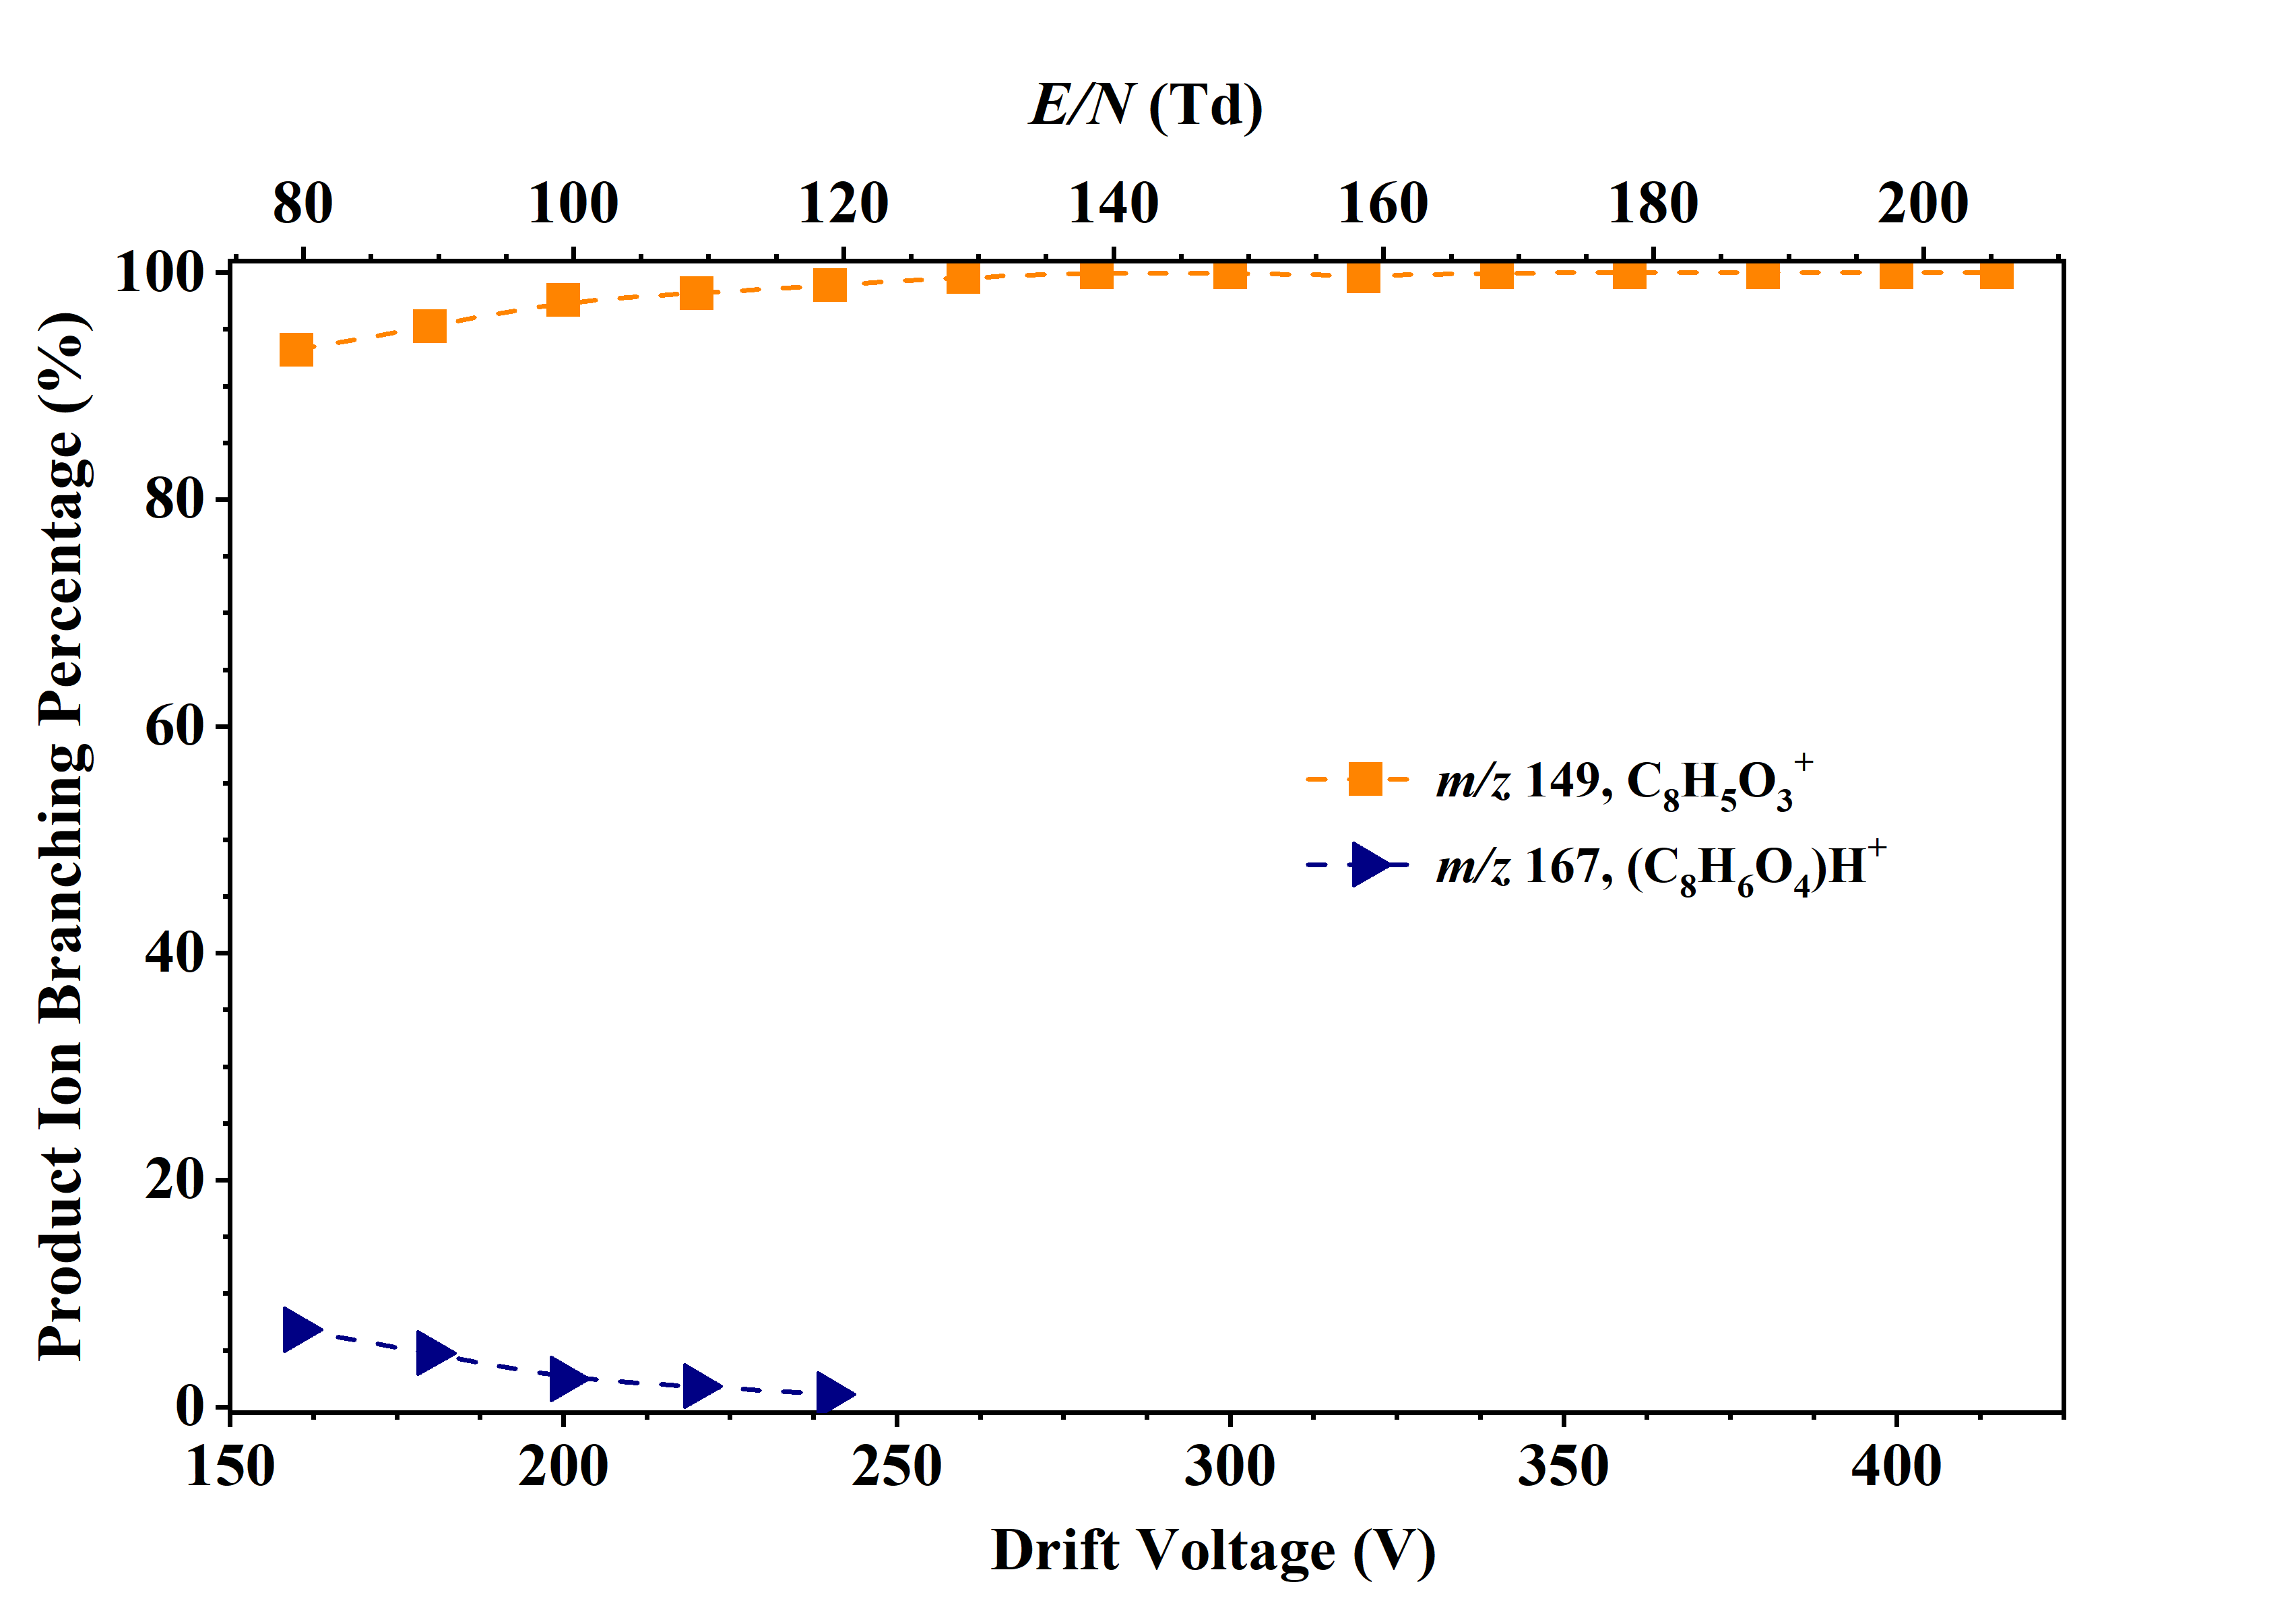
\includegraphics[height=0.4\textheight]{pics/Pacid-BR.png}
\caption{Percentage product ion distribution resulting from the reaction of phthalic acid with H\textsubscript{3}O\textsuperscript{+} as a function of the drift voltage and the reduced electric field in the range from 80 to 205 Td.}
\label{fig:PAcid}
\end{figure}


\begin{figure}
\centering
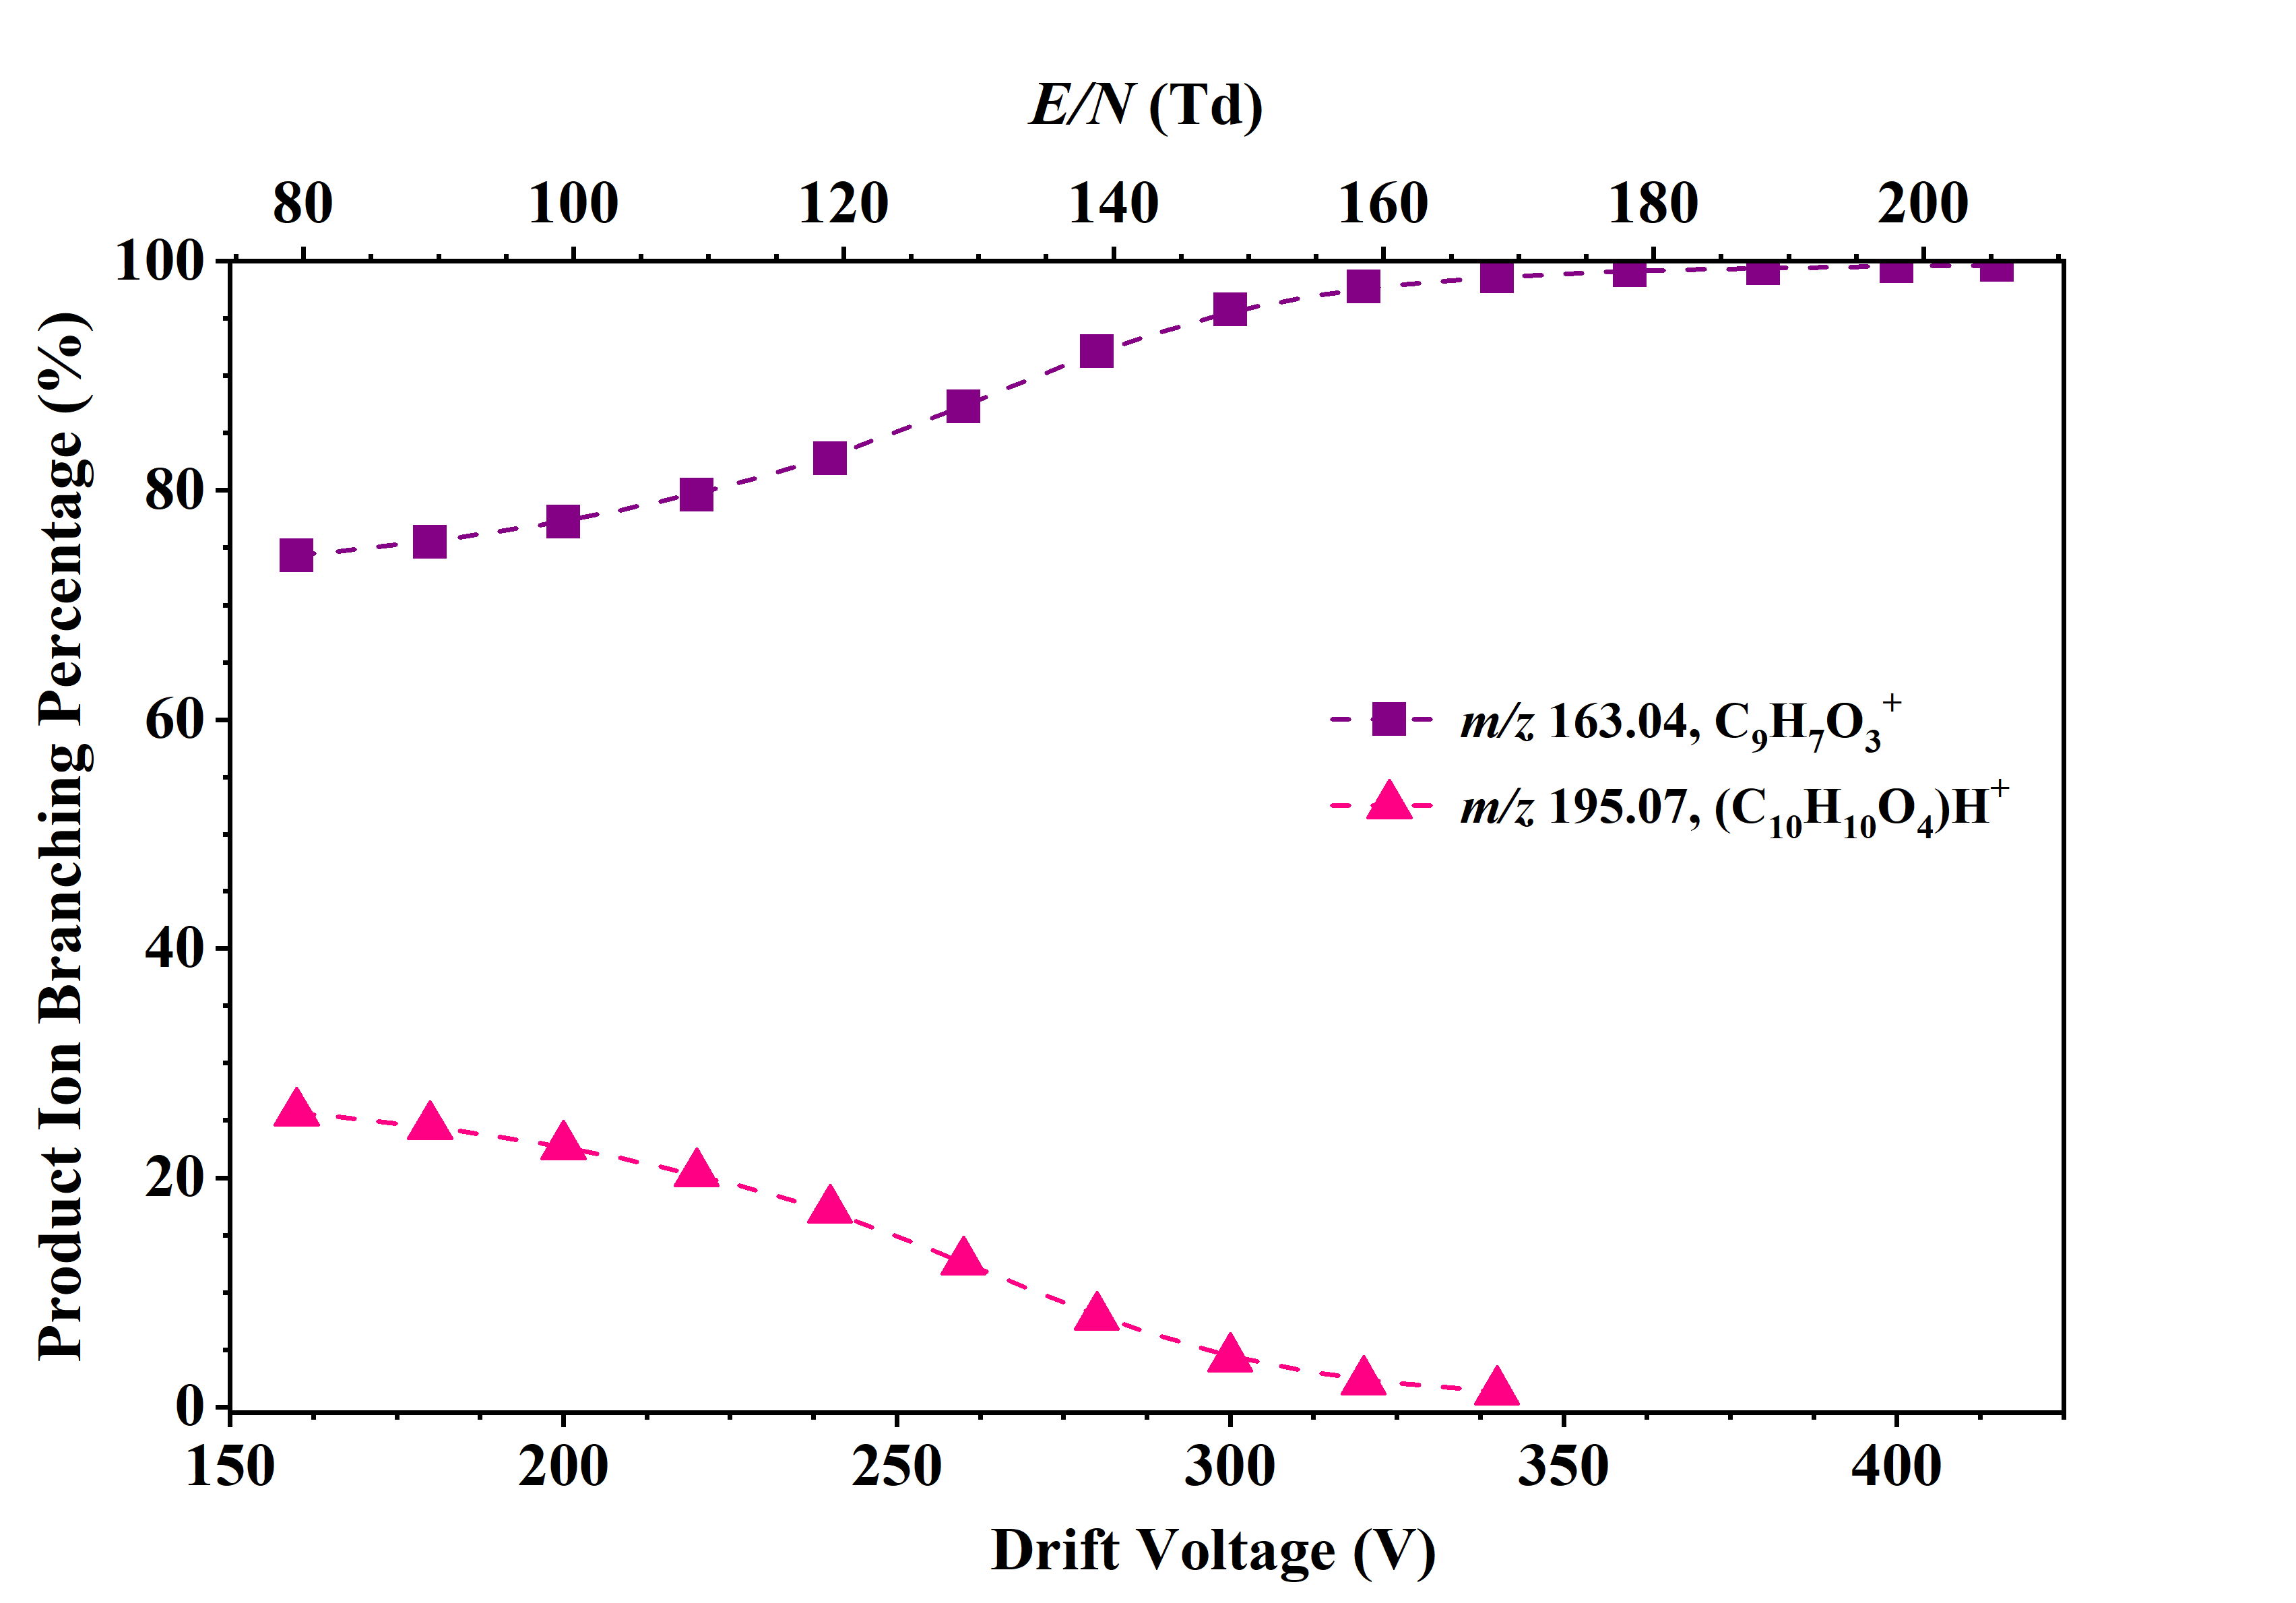
\includegraphics[height=0.4\textheight]{pics/DMP-BR.png}
\caption{Percentage product ion distribution resulting from the reaction of DMP with H\textsubscript{3}O\textsuperscript{+} as a function of the drift voltage and the reduced electric field in the range from 80 to 205 Td.}
\label{fig:DMP_fs}
\end{figure}


\begin{figure}
\centering
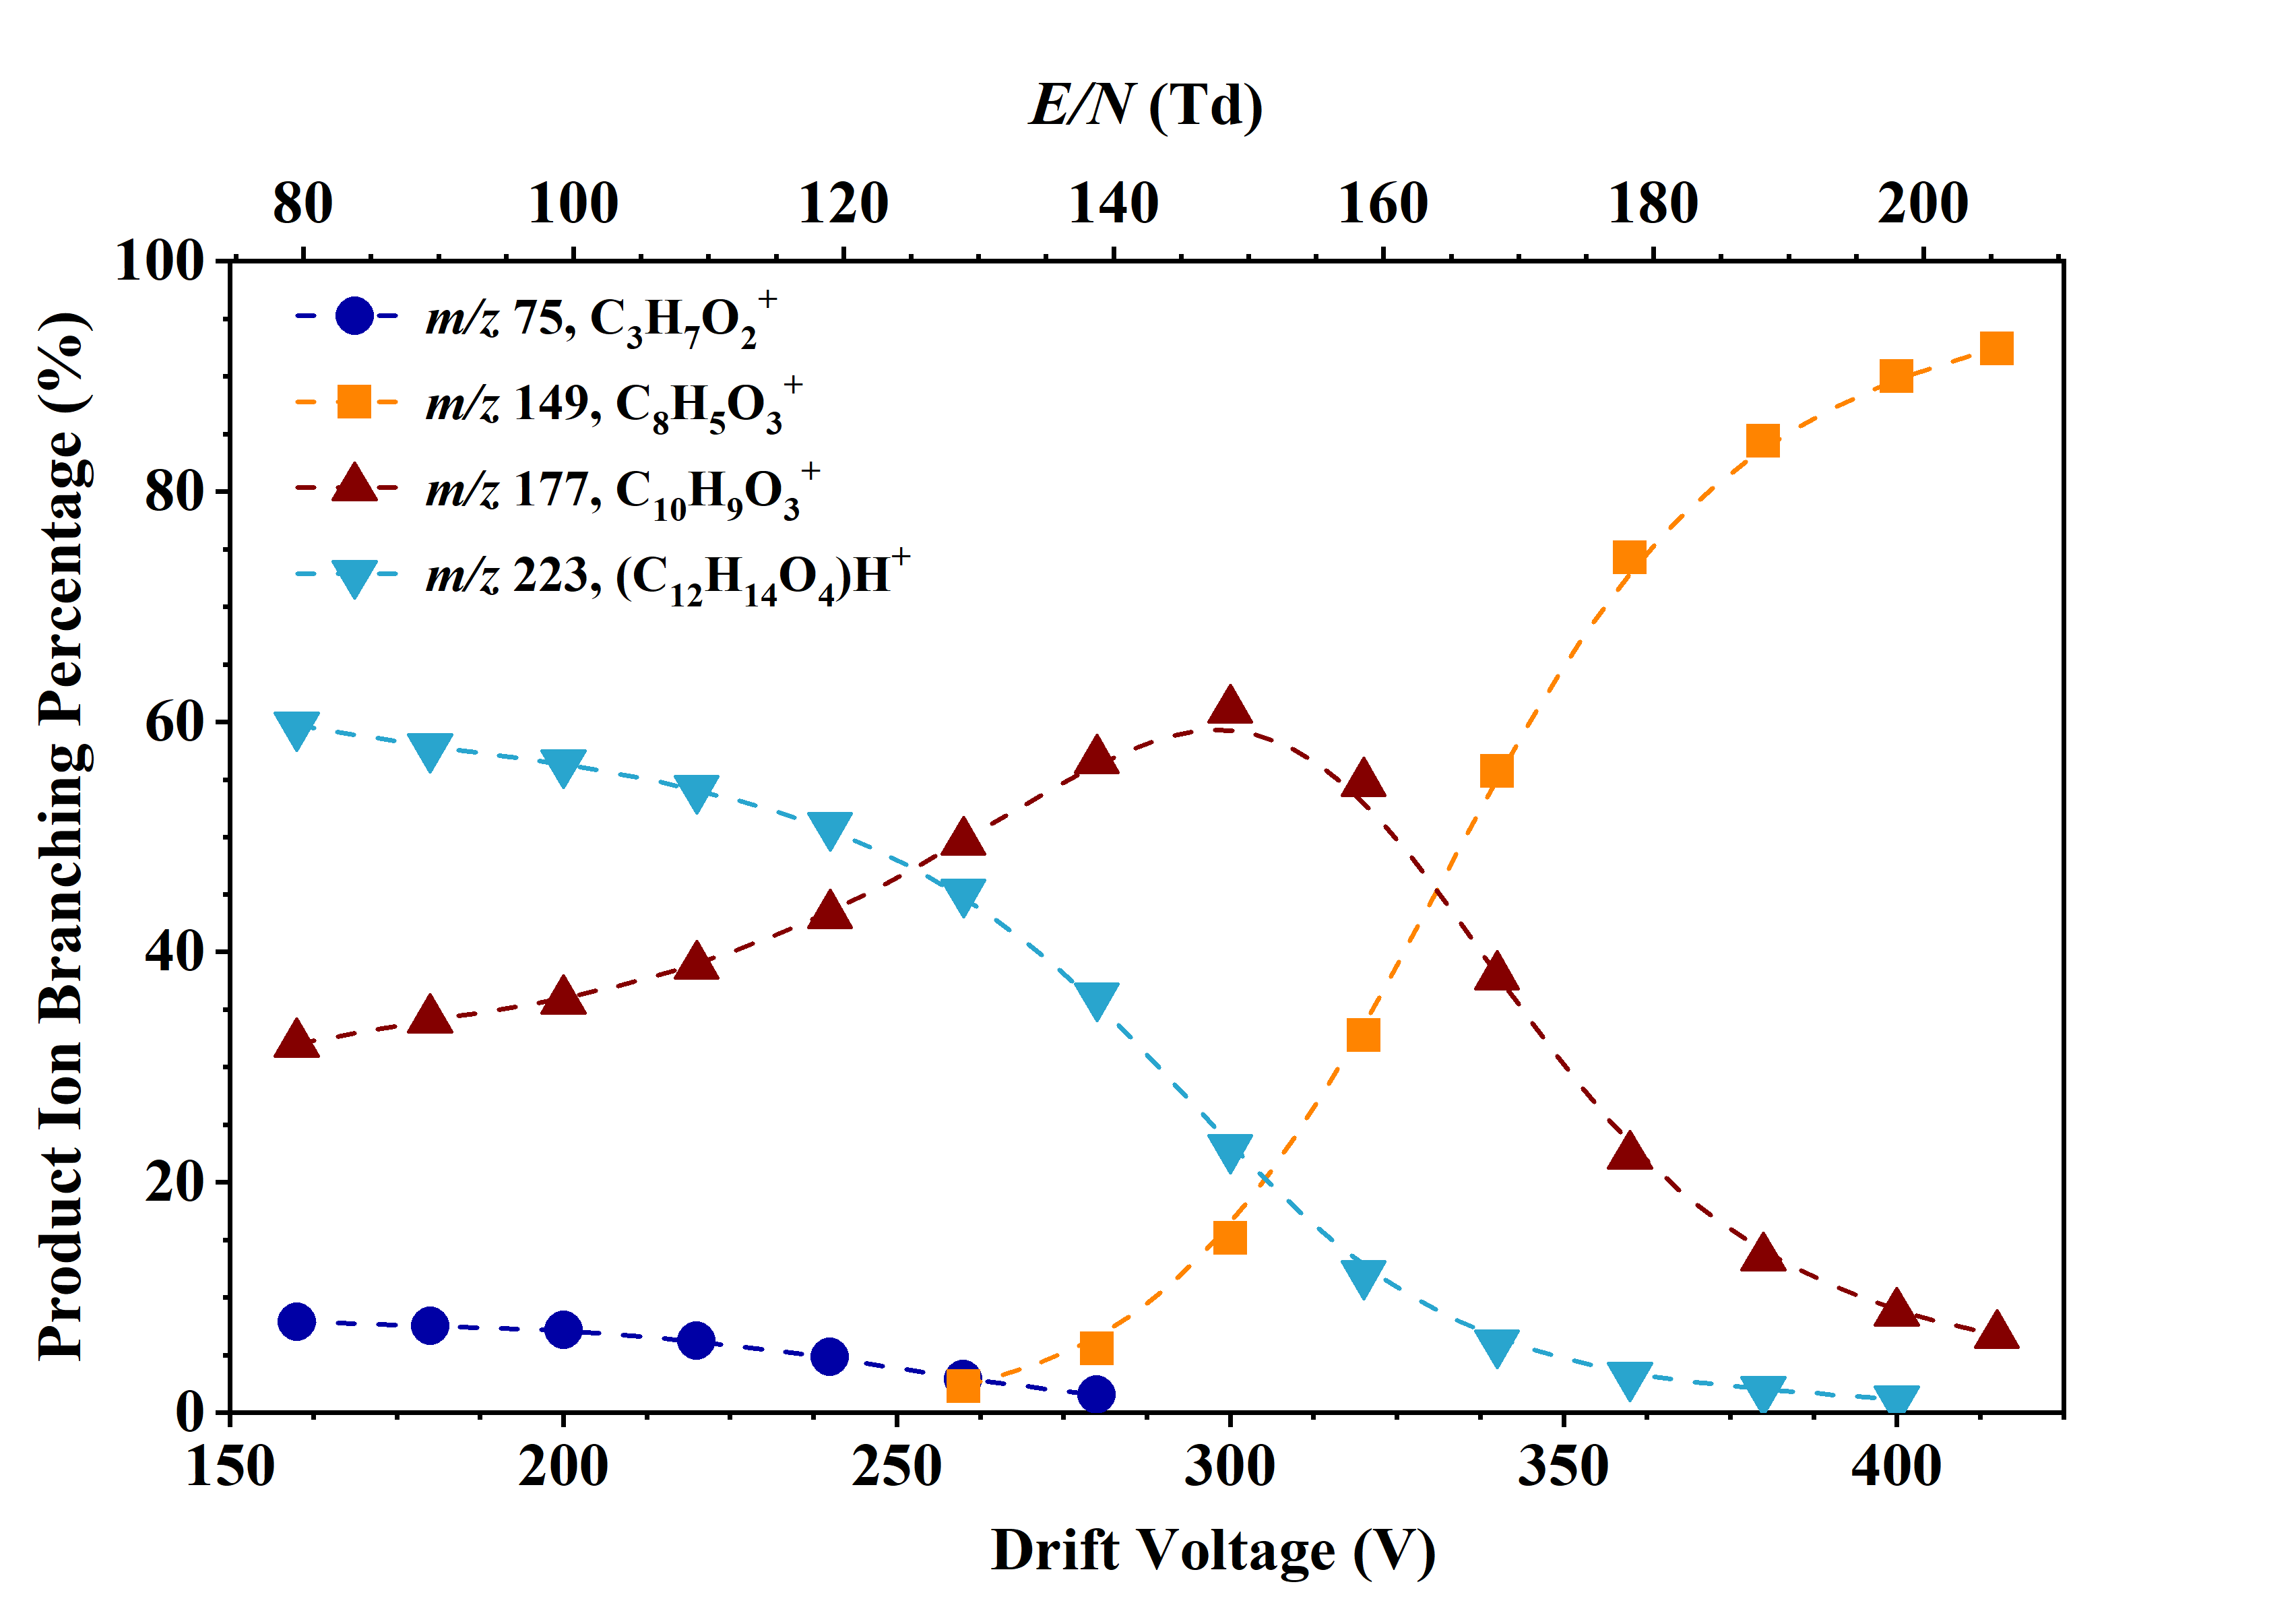
\includegraphics[height=0.4\textheight]{pics/DEP-BR.png}
\caption{Percentage product ion distribution resulting from the reaction of DEP with H\textsubscript{3}O\textsuperscript{+} as a function of the drift voltage and the reduced electric field in the range from 80 to 205 Td.}
\label{fig:DEP_fs}
\end{figure}


\begin{figure}
\centering
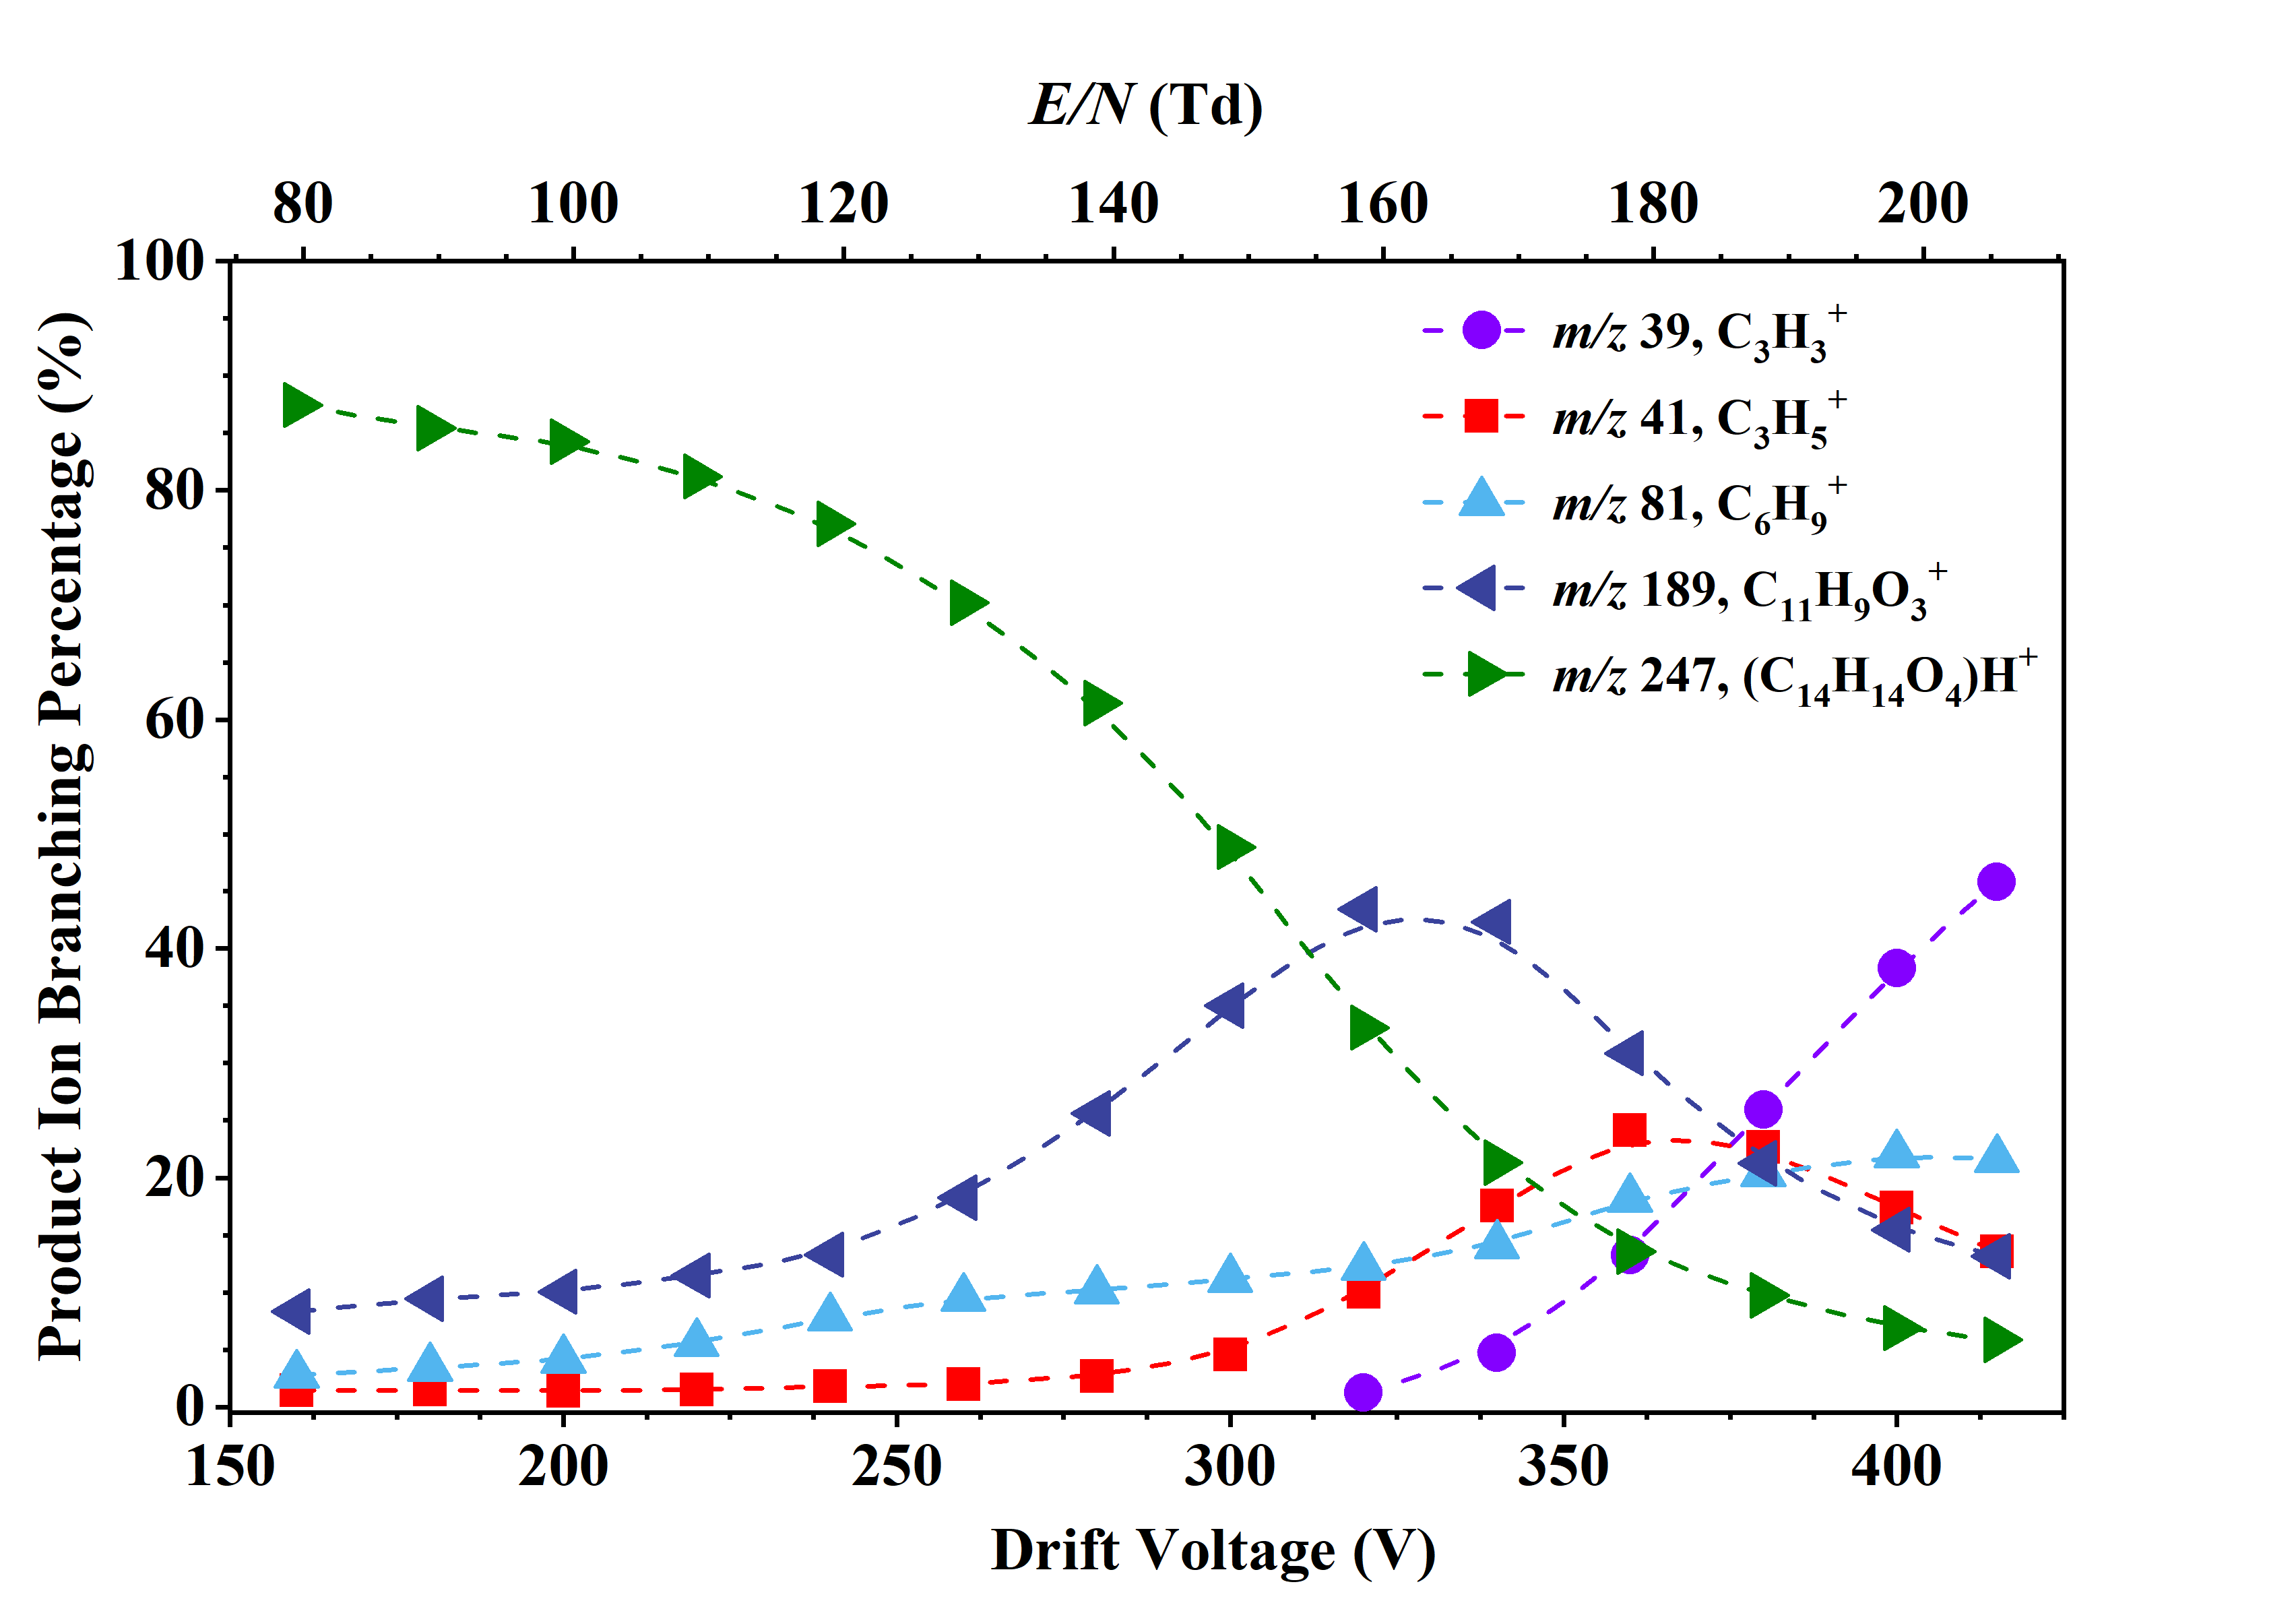
\includegraphics[height=0.4\textheight]{pics/DAP-BR.png}
\caption{Percentage product ion distribution resulting from the reaction of DAP with H\textsubscript{3}O\textsuperscript{+} as a function of the drift voltage and the reduced electric field in the range from 80 to 205 Td.}
\label{fig:DAP_fs}
\end{figure}


\begin{figure}
\centering
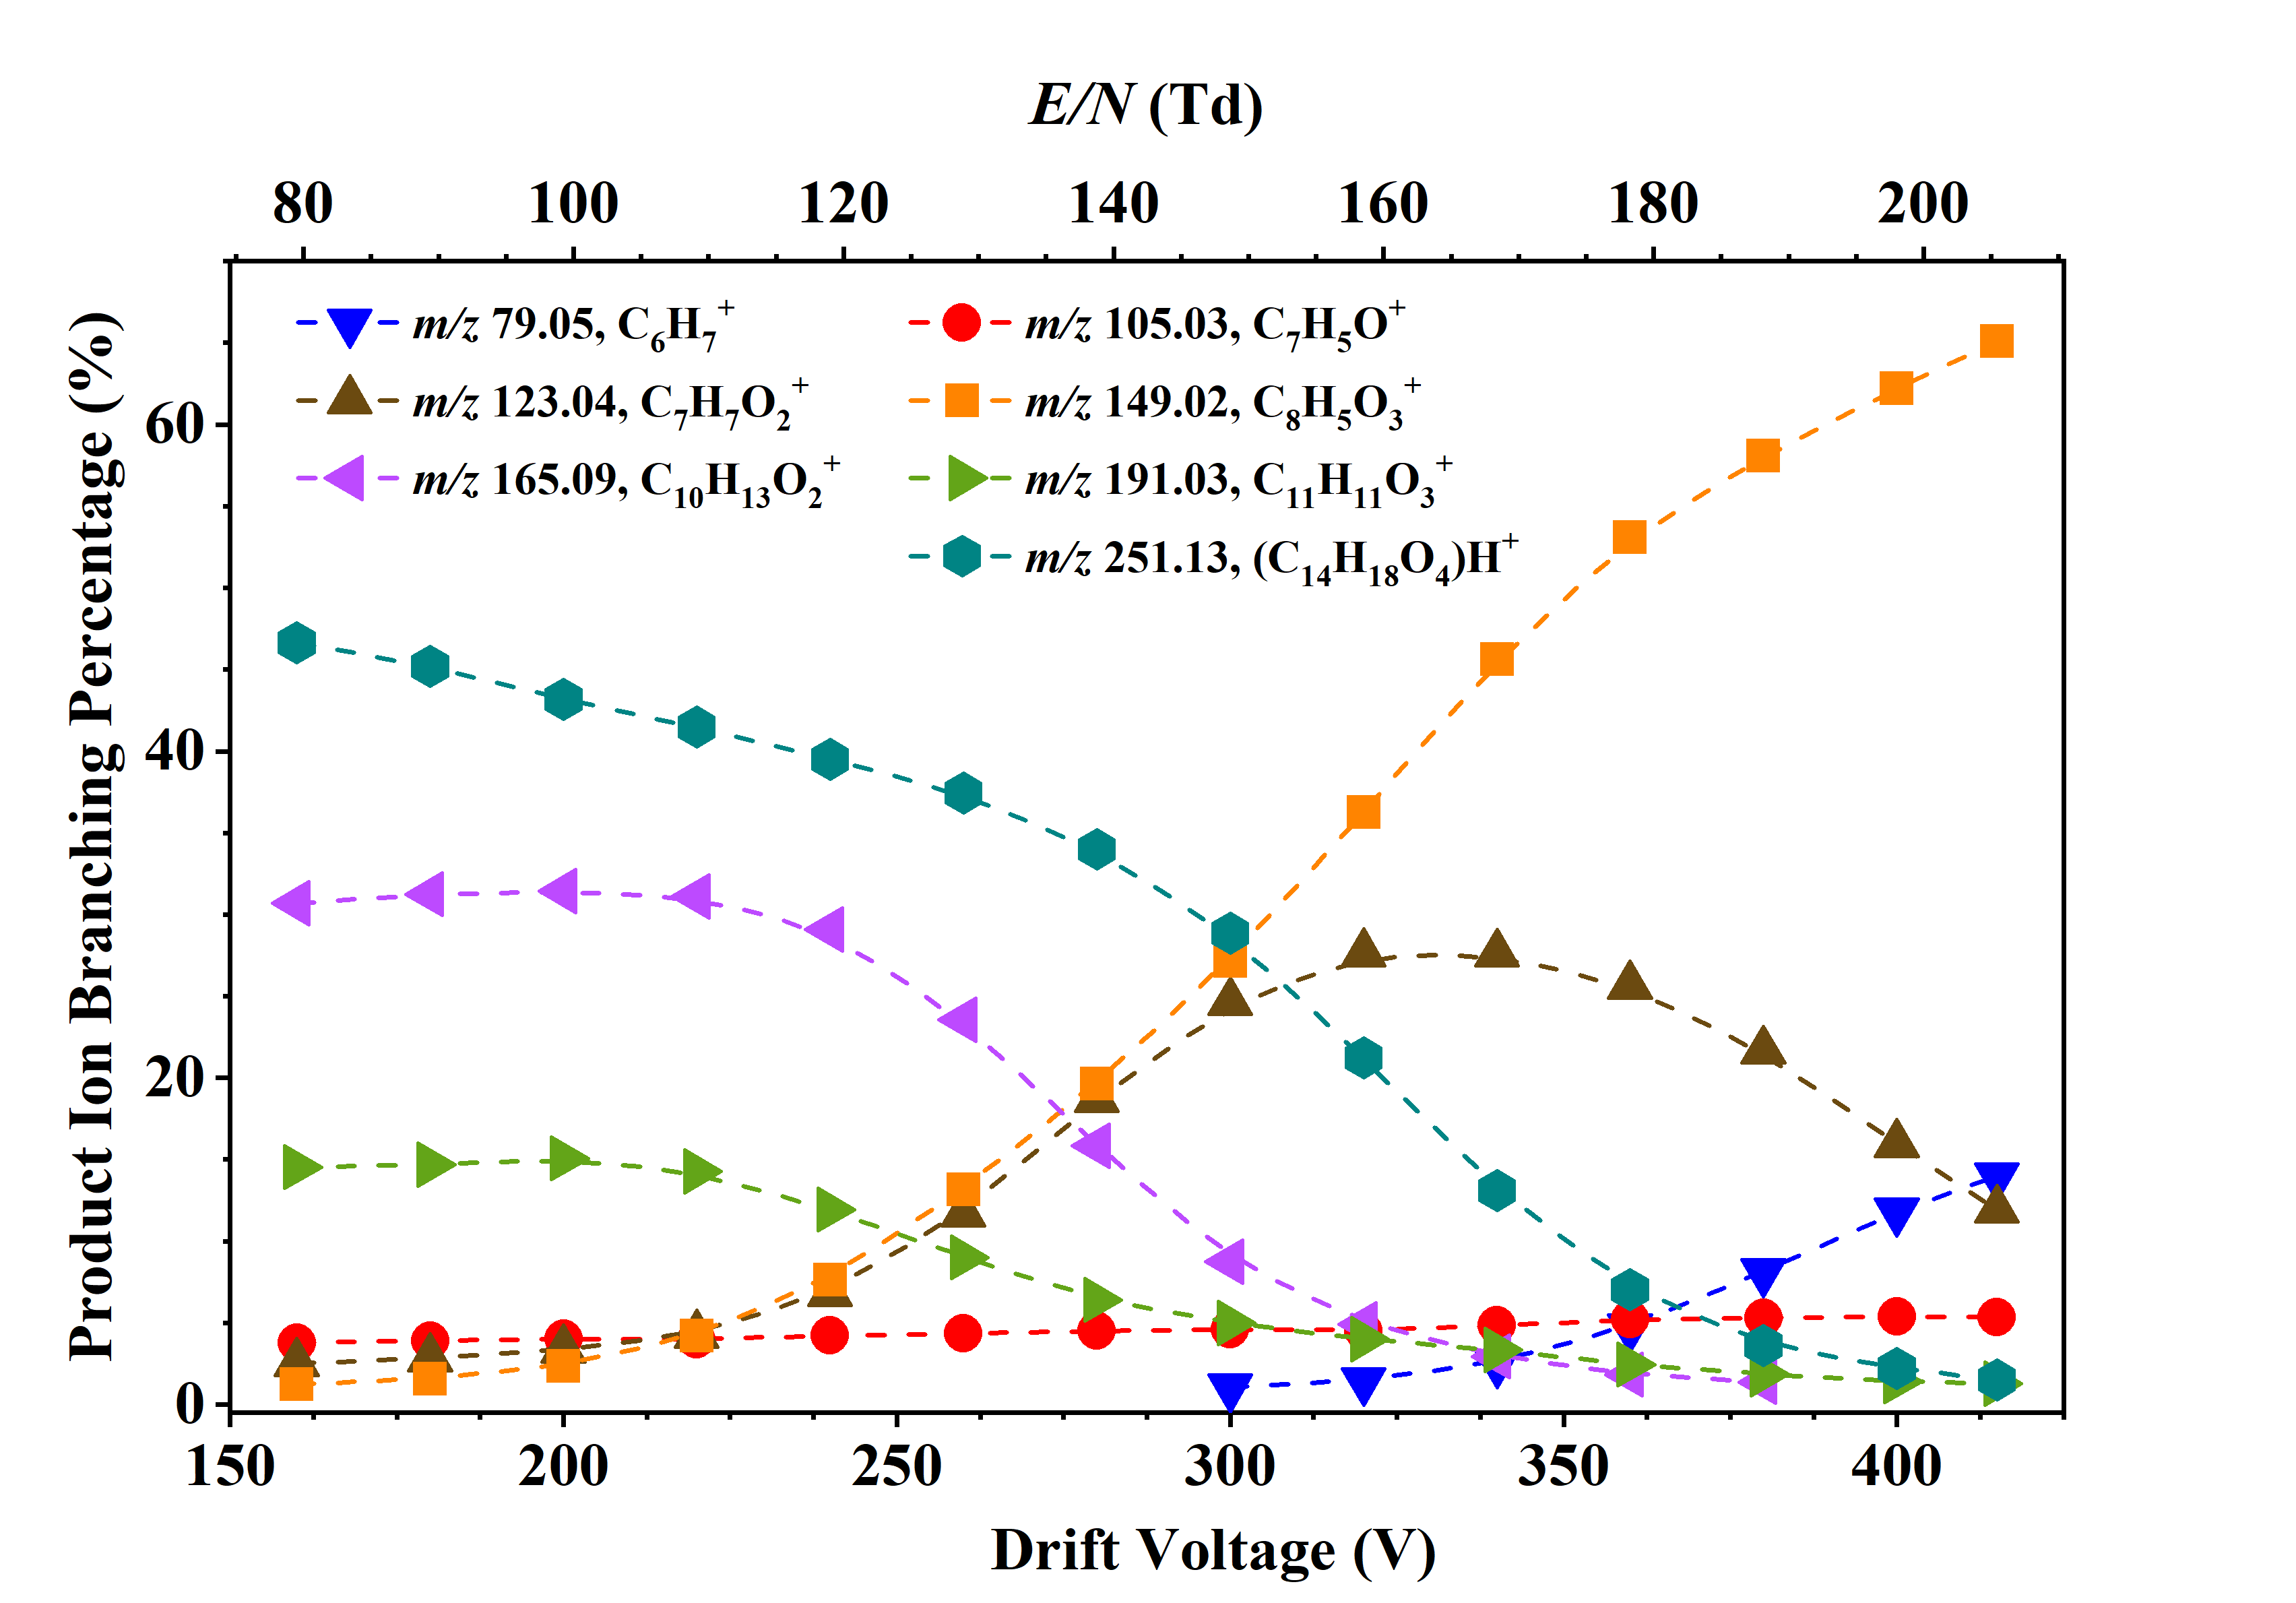
\includegraphics[height=0.4\textheight]{pics/DPP-BR.png}
\caption{Percentage product ion distribution resulting from the reaction of DPP with H\textsubscript{3}O\textsuperscript{+} as a function of the drift voltage and the reduced electric field in the range from 80 to 205 Td.}
\label{fig:DPP_fs}
\end{figure}


\begin{figure}
\centering
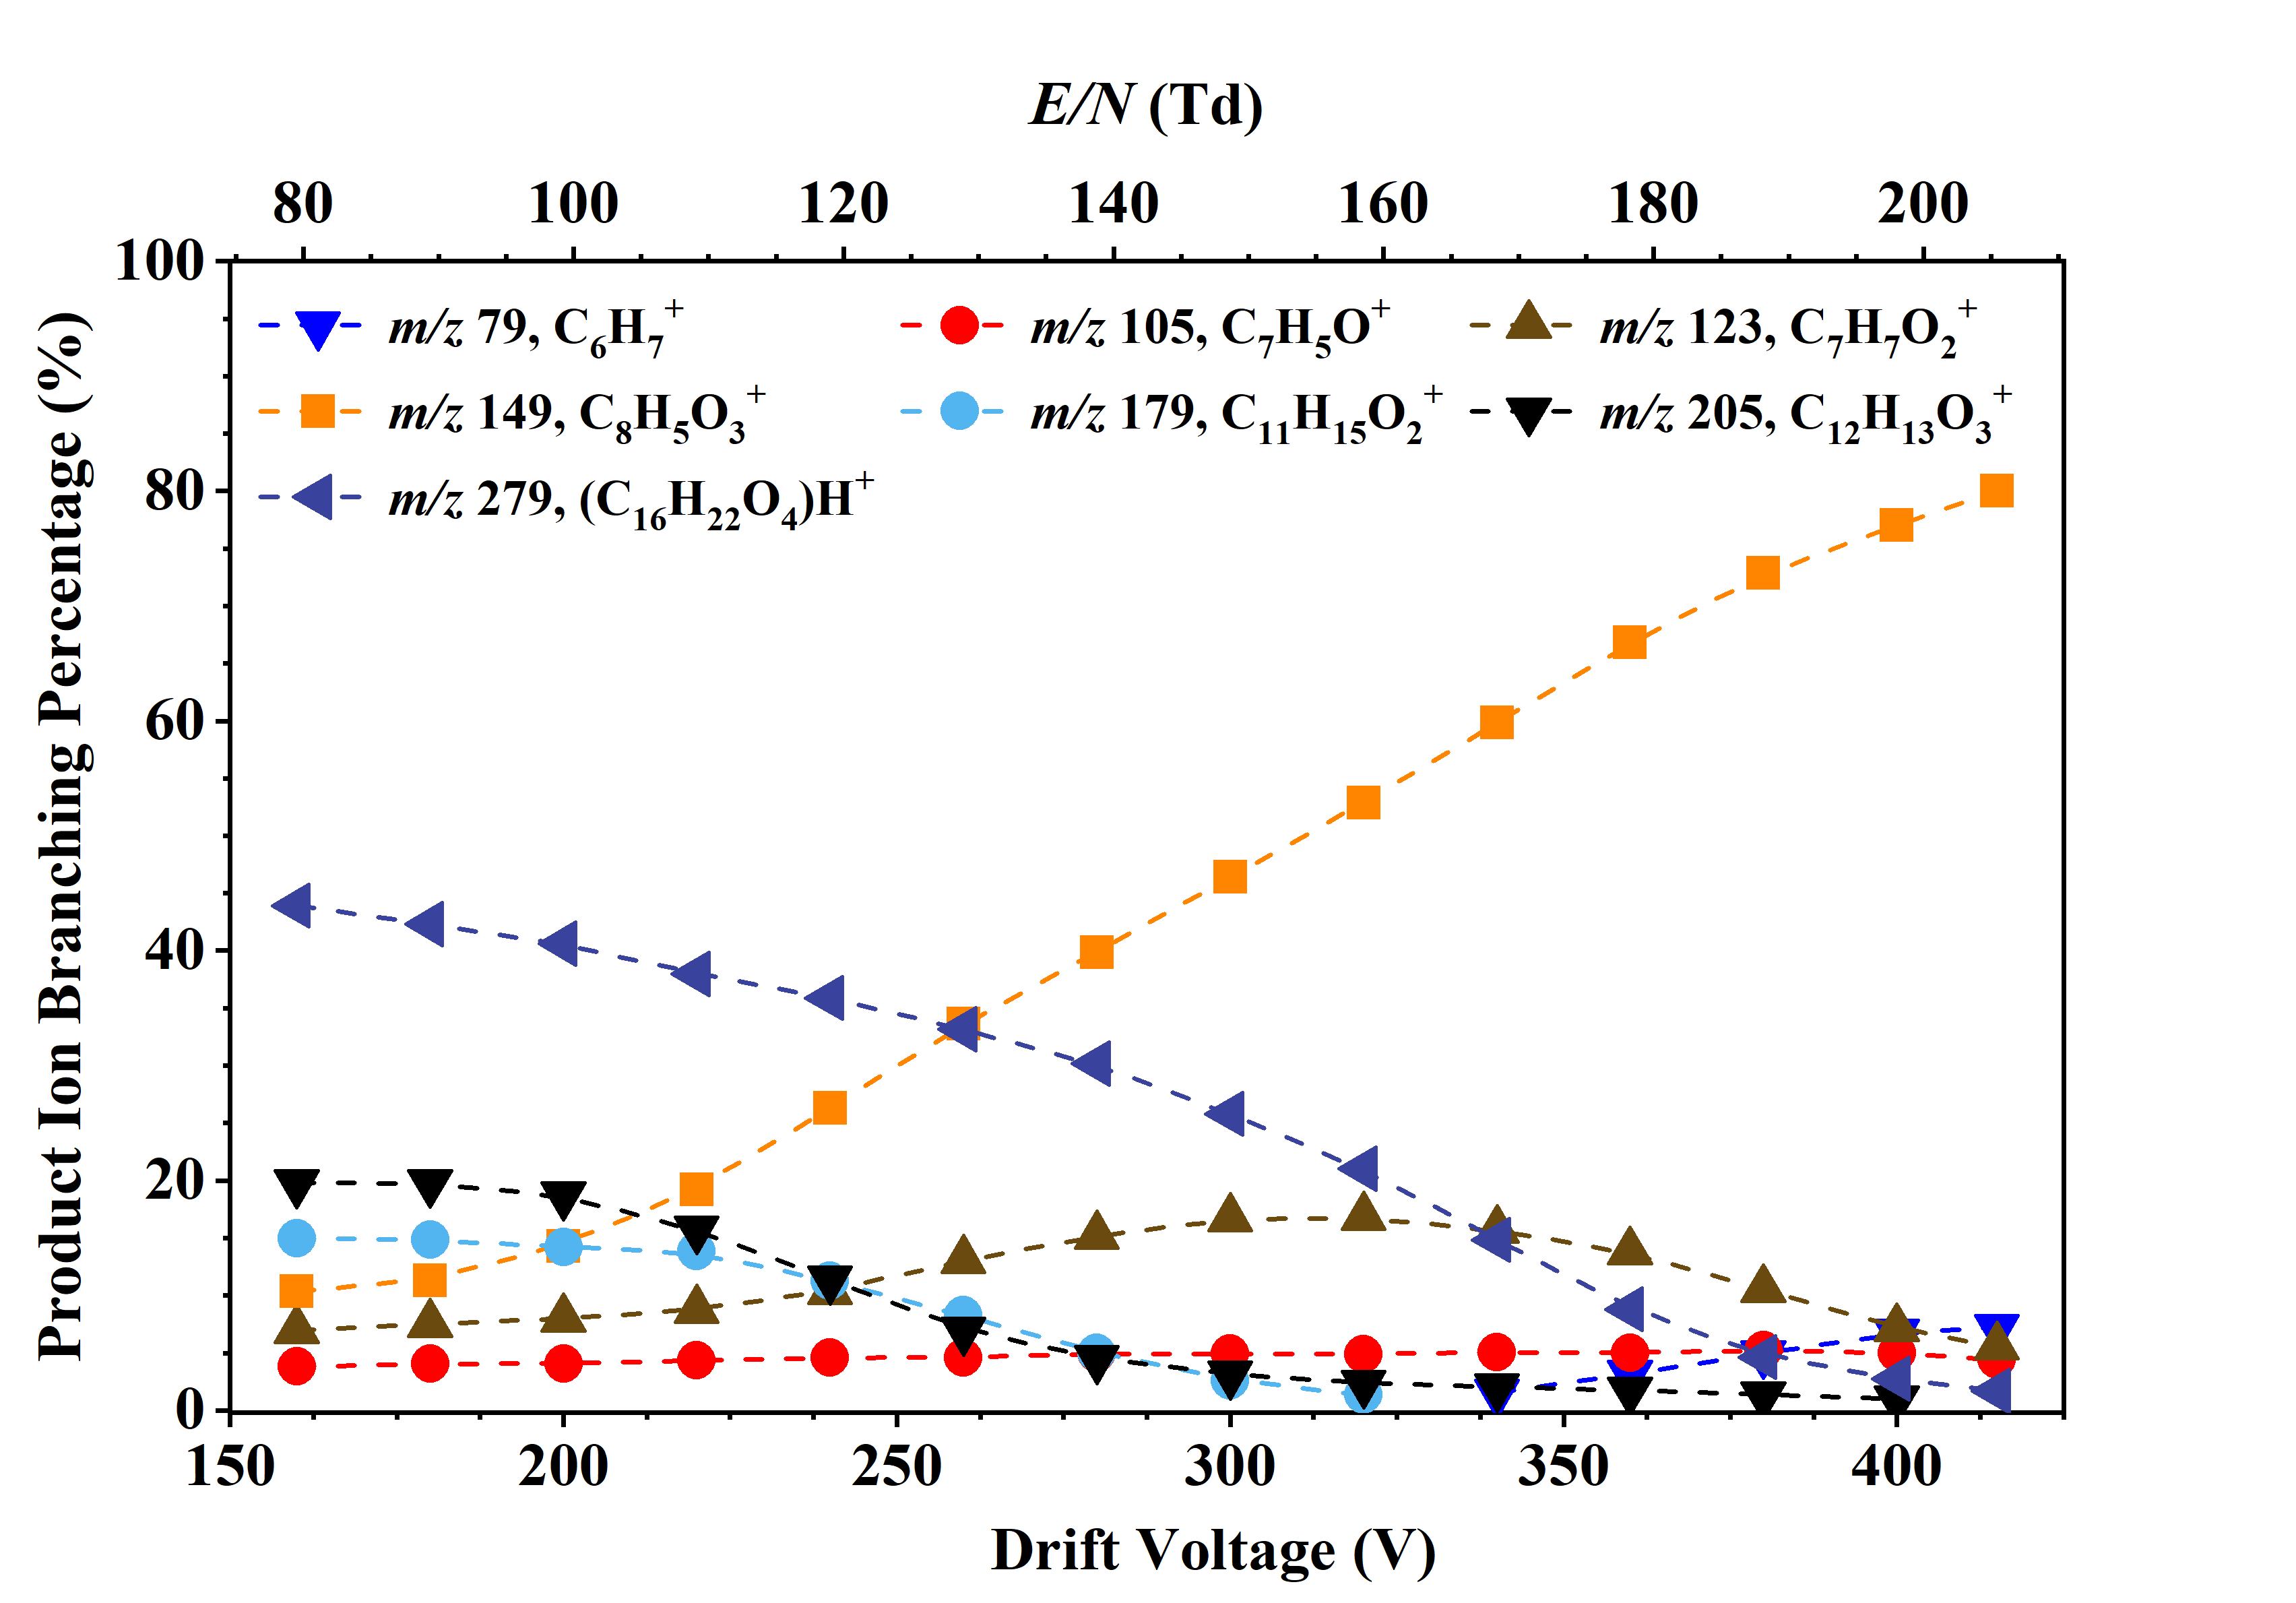
\includegraphics[height=0.4\textheight]{pics/DBP-BR.png}
\caption{Percentage product ion distribution resulting from the reaction of DBP with H\textsubscript{3}O\textsuperscript{+} as a function of the drift voltage and the reduced electric field in the range from 80 to 205 Td.}
\label{fig:DBP_fs}
\end{figure}


\begin{figure}
\centering
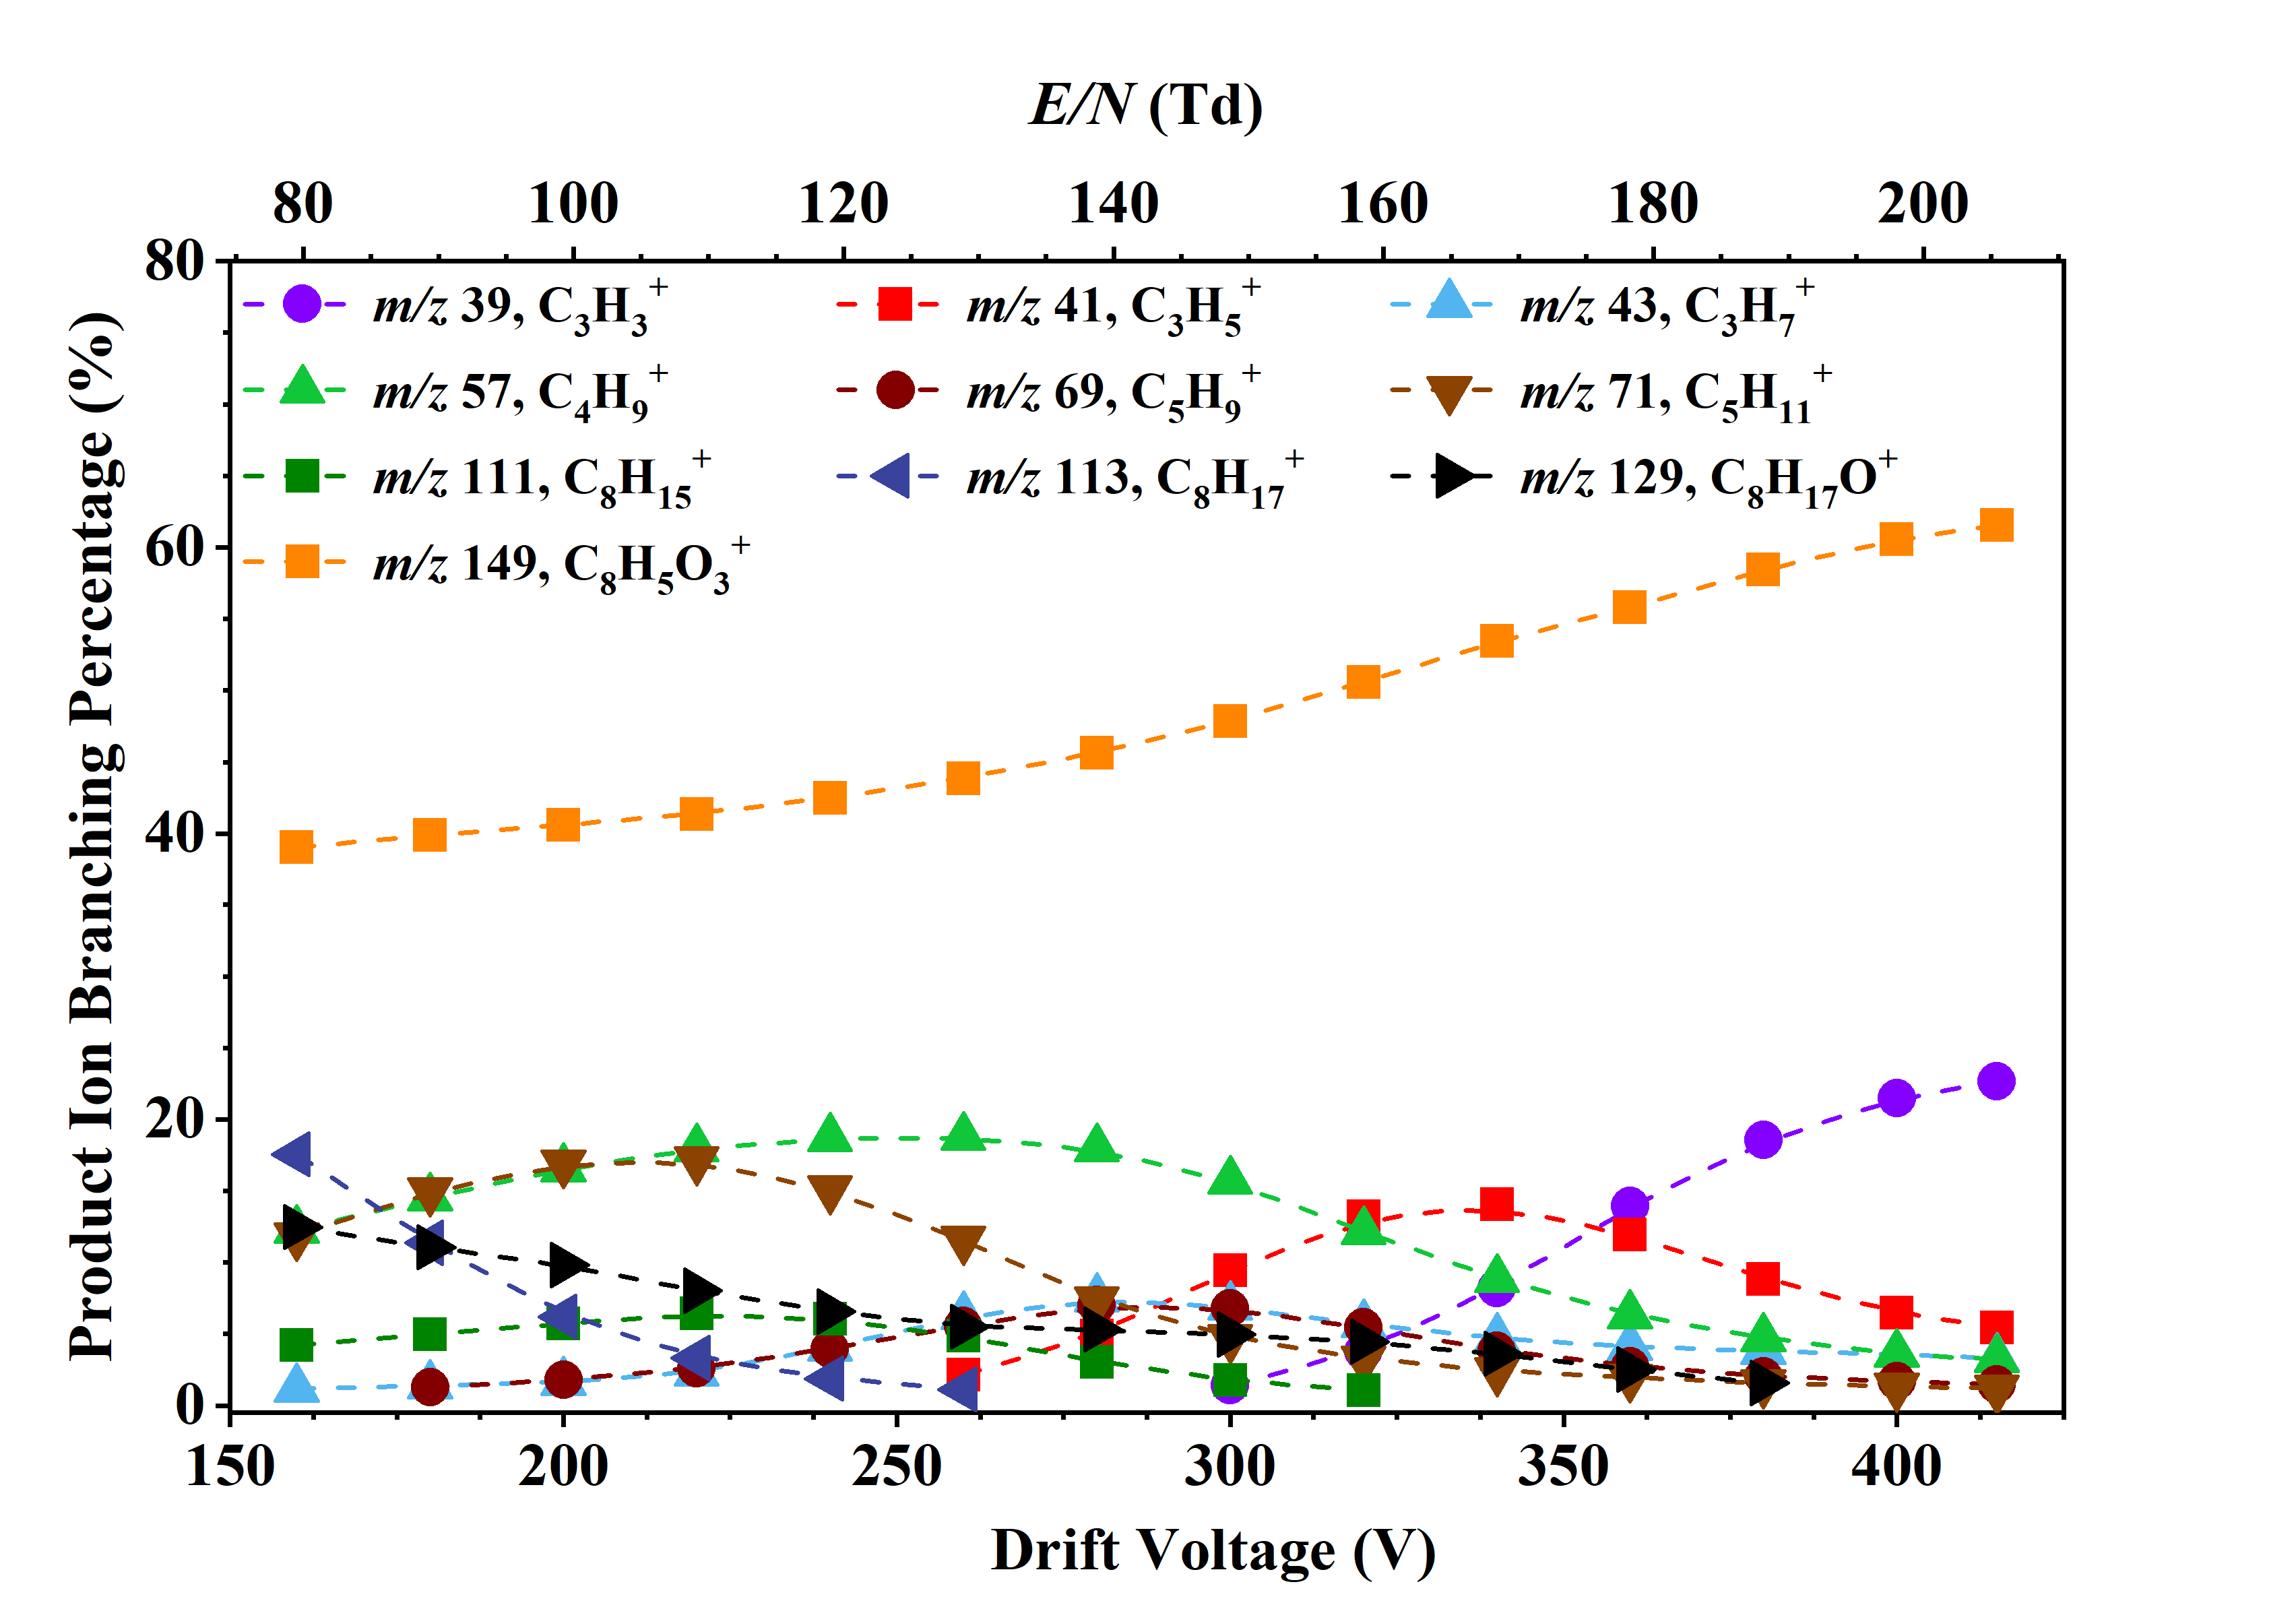
\includegraphics[height=0.4\textheight]{pics/MEHP-BR.png}
\caption{Percentage product ion distribution resulting from the reaction of MEHP with H\textsubscript{3}O\textsuperscript{+} as a function of the drift voltage and the reduced electric field in the range from 80 to 205 Td.}
\label{fig:MEHP_fs}
\end{figure}


\begin{figure}
\centering
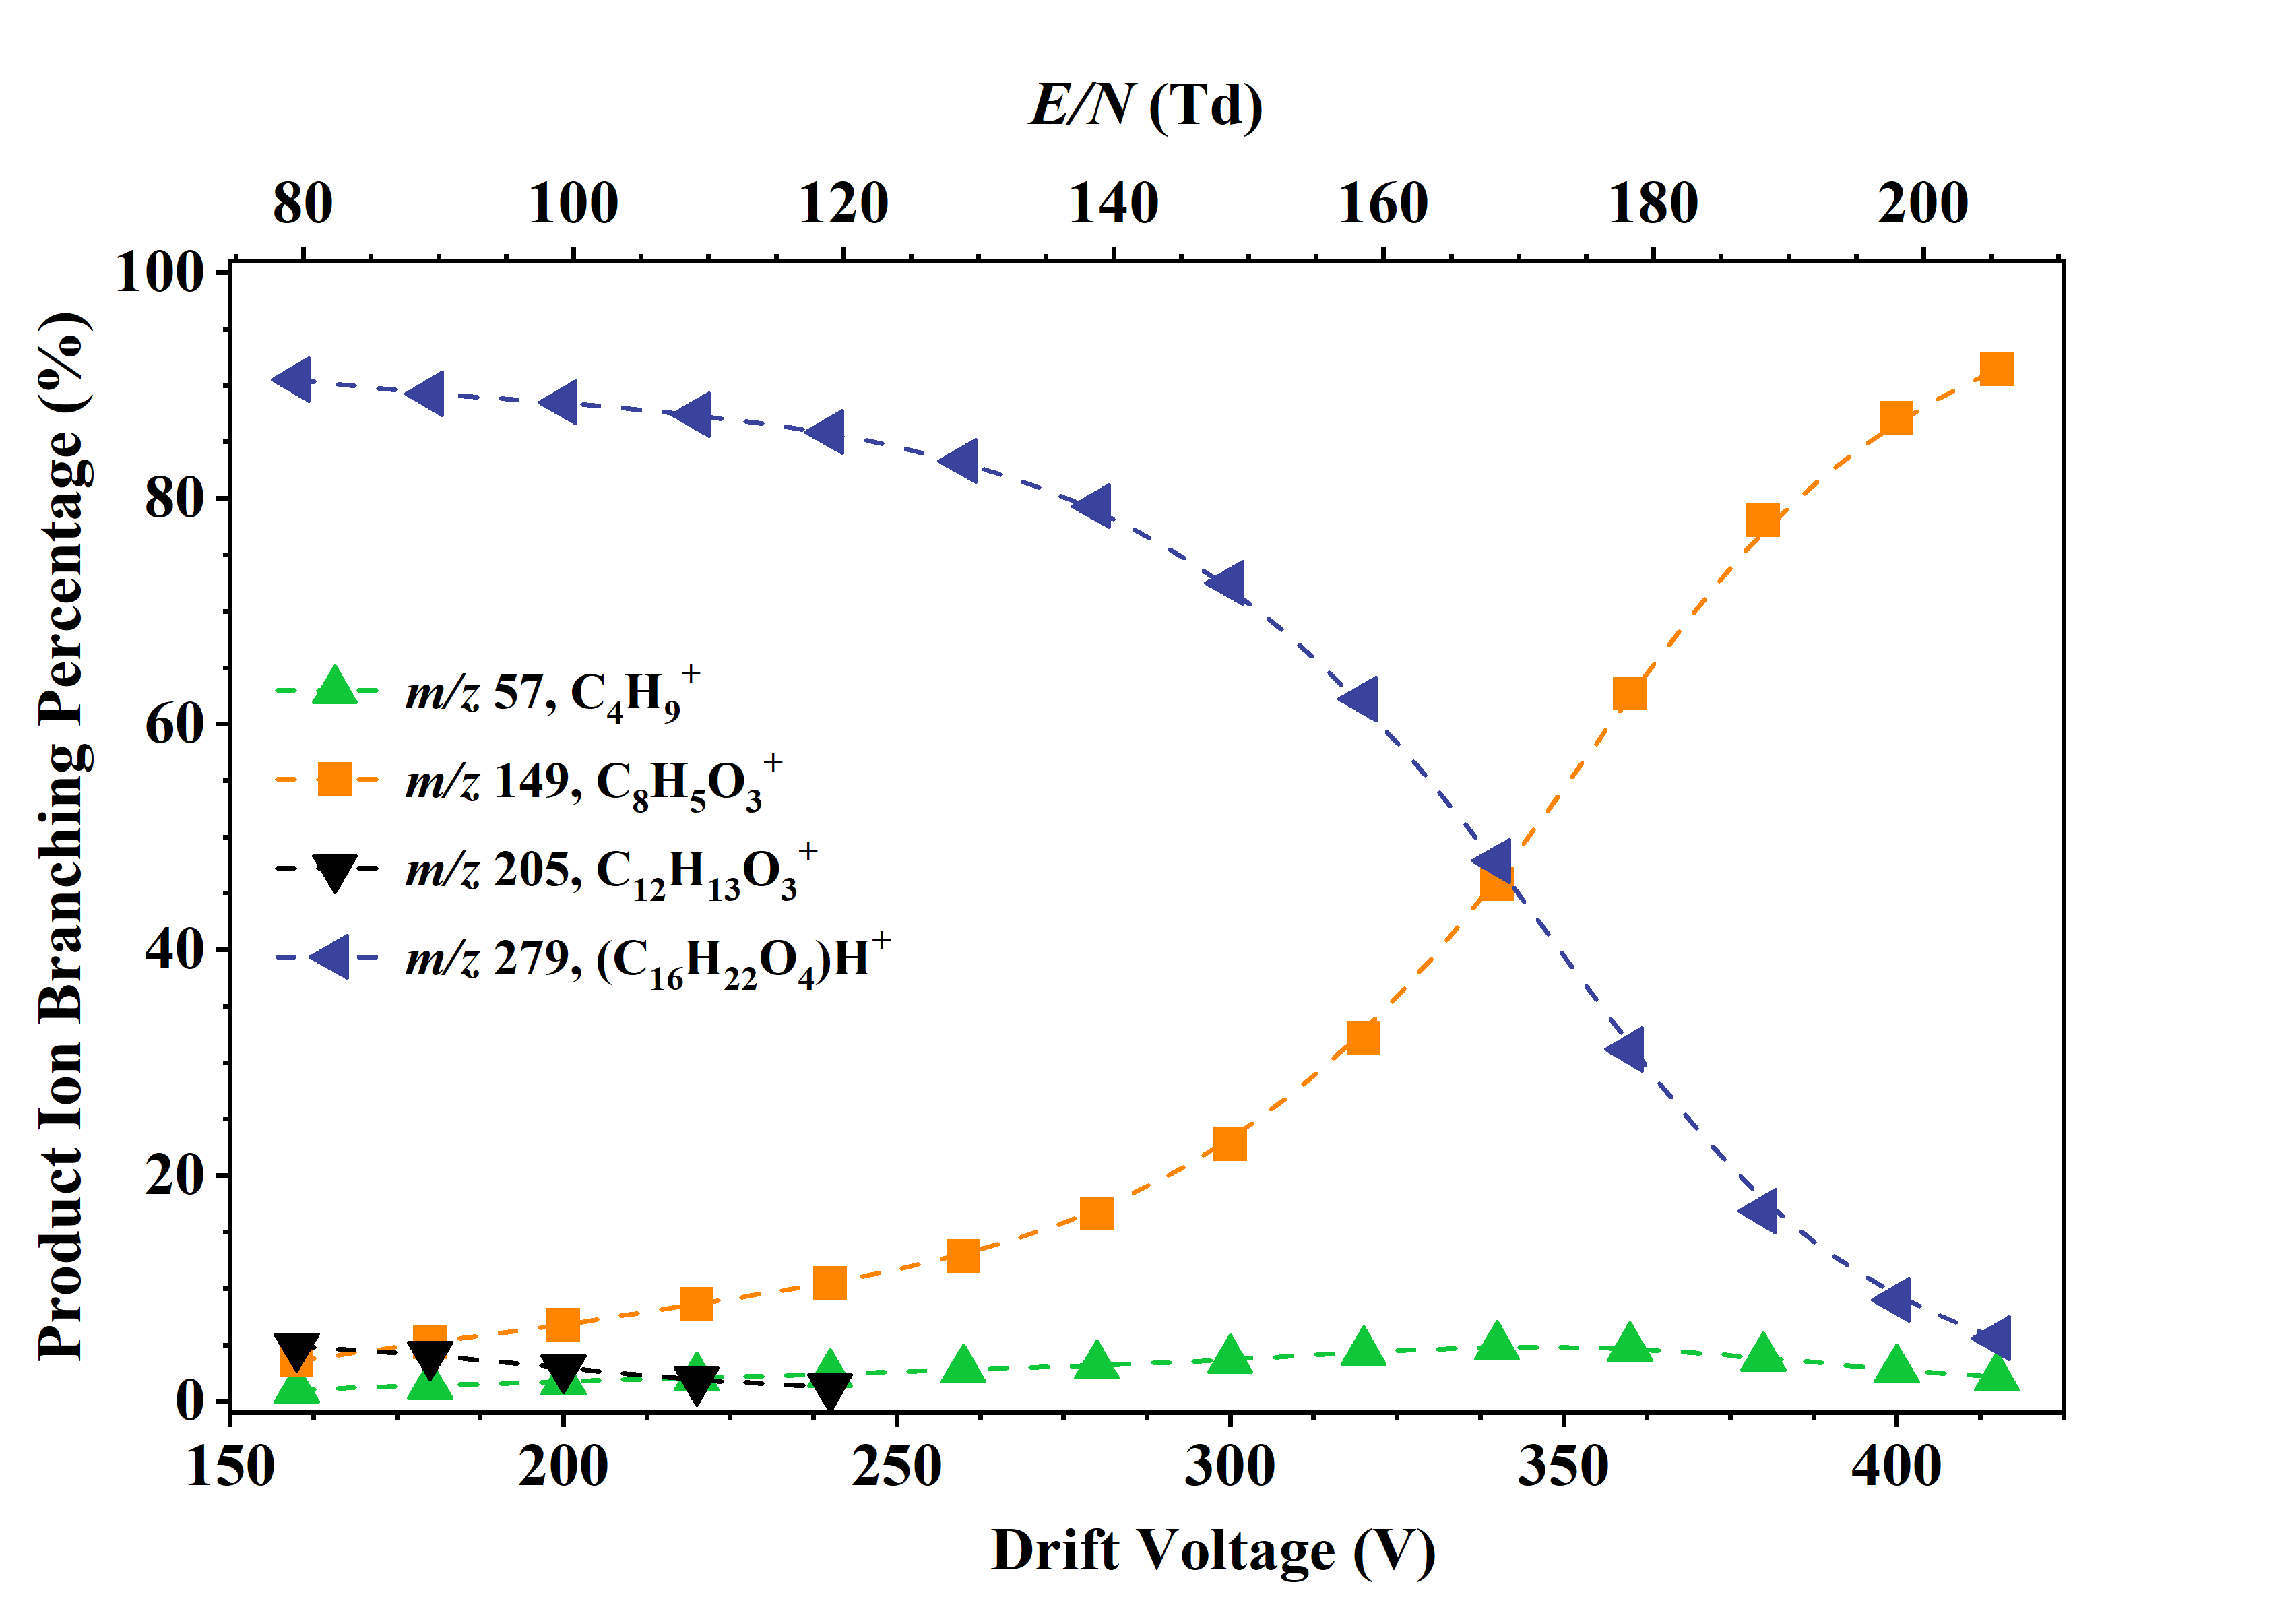
\includegraphics[height=0.4\textheight]{pics/DiBP-BR.png}
\caption{Percentage product ion distribution resulting from the reaction of DiBP with H\textsubscript{3}O\textsuperscript{+} as a function of the drift voltage and the reduced electric field in the range from 80 to 205 Td.}
\label{fig:DiBP_fs}
\end{figure}

\begin{figure}
\centering
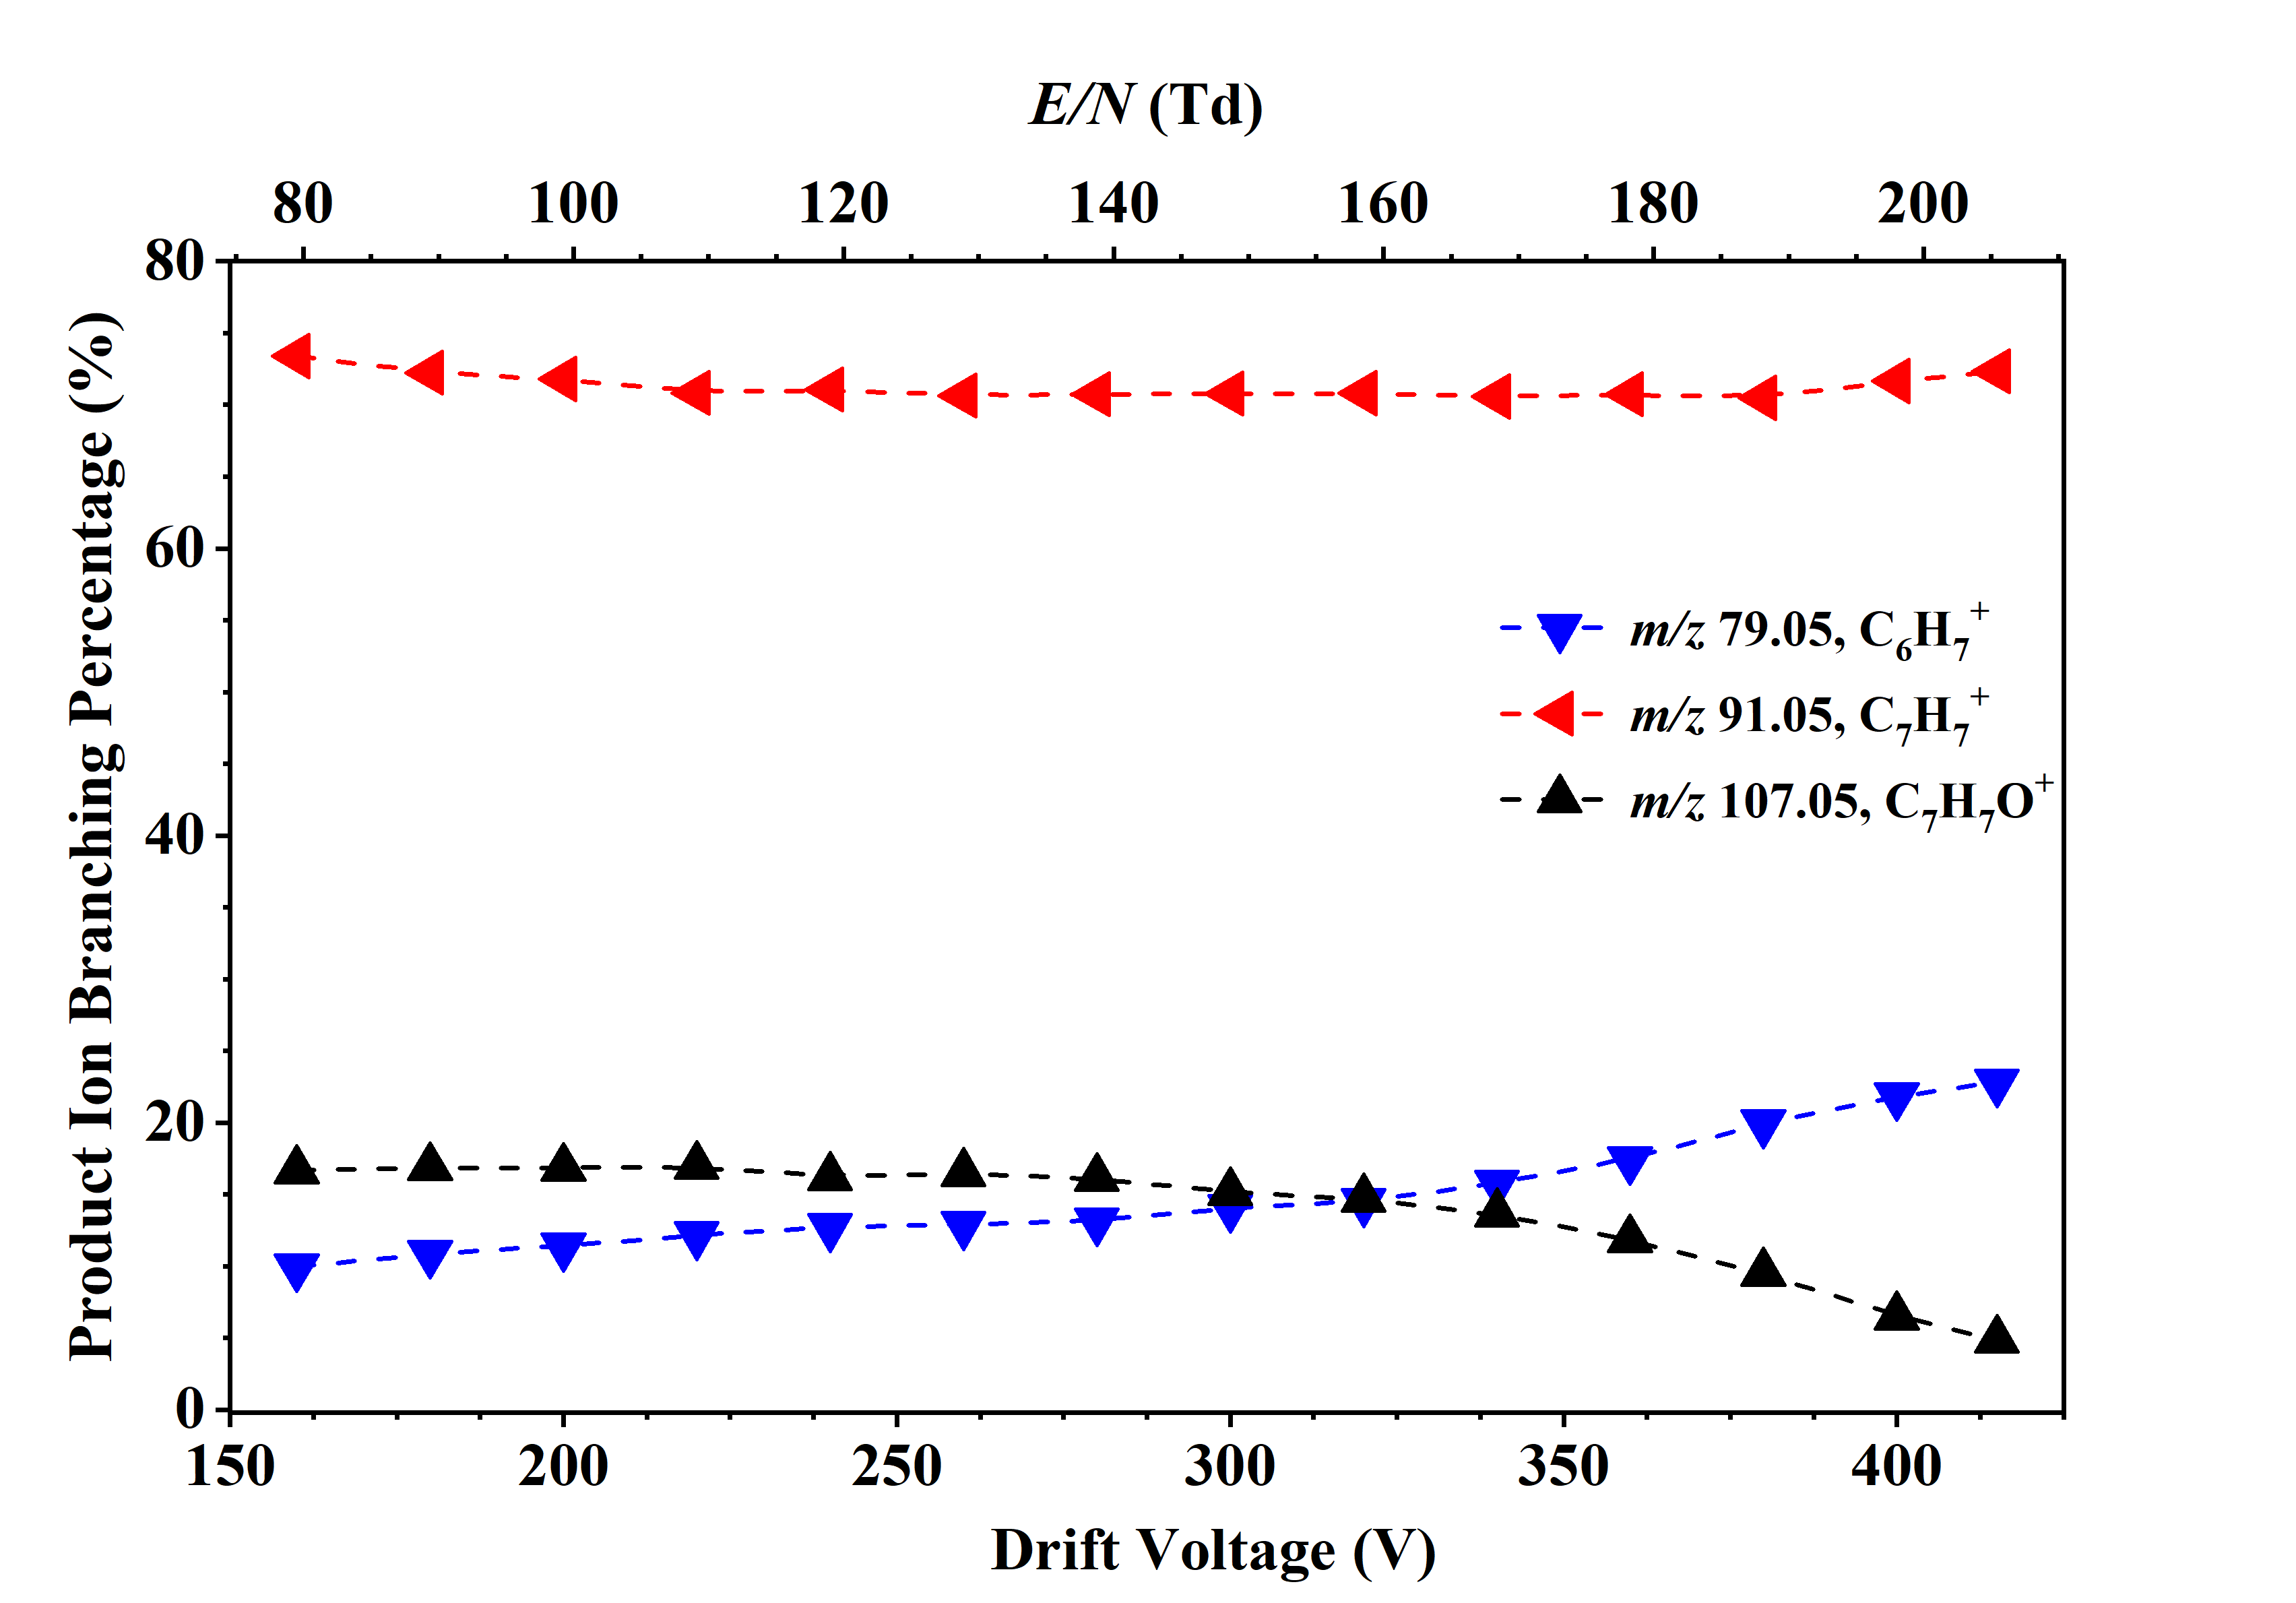
\includegraphics[height=0.4\textheight]{pics/BBP-BR.png}
\caption{Percentage product ion distribution resulting from the reaction of BBP with H\textsubscript{3}O\textsuperscript{+} as a function of the drift voltage and the reduced electric field in the range from 80 to 205 Td.}
\label{fig:BBP_fs}
\end{figure}

\begin{figure}
\centering
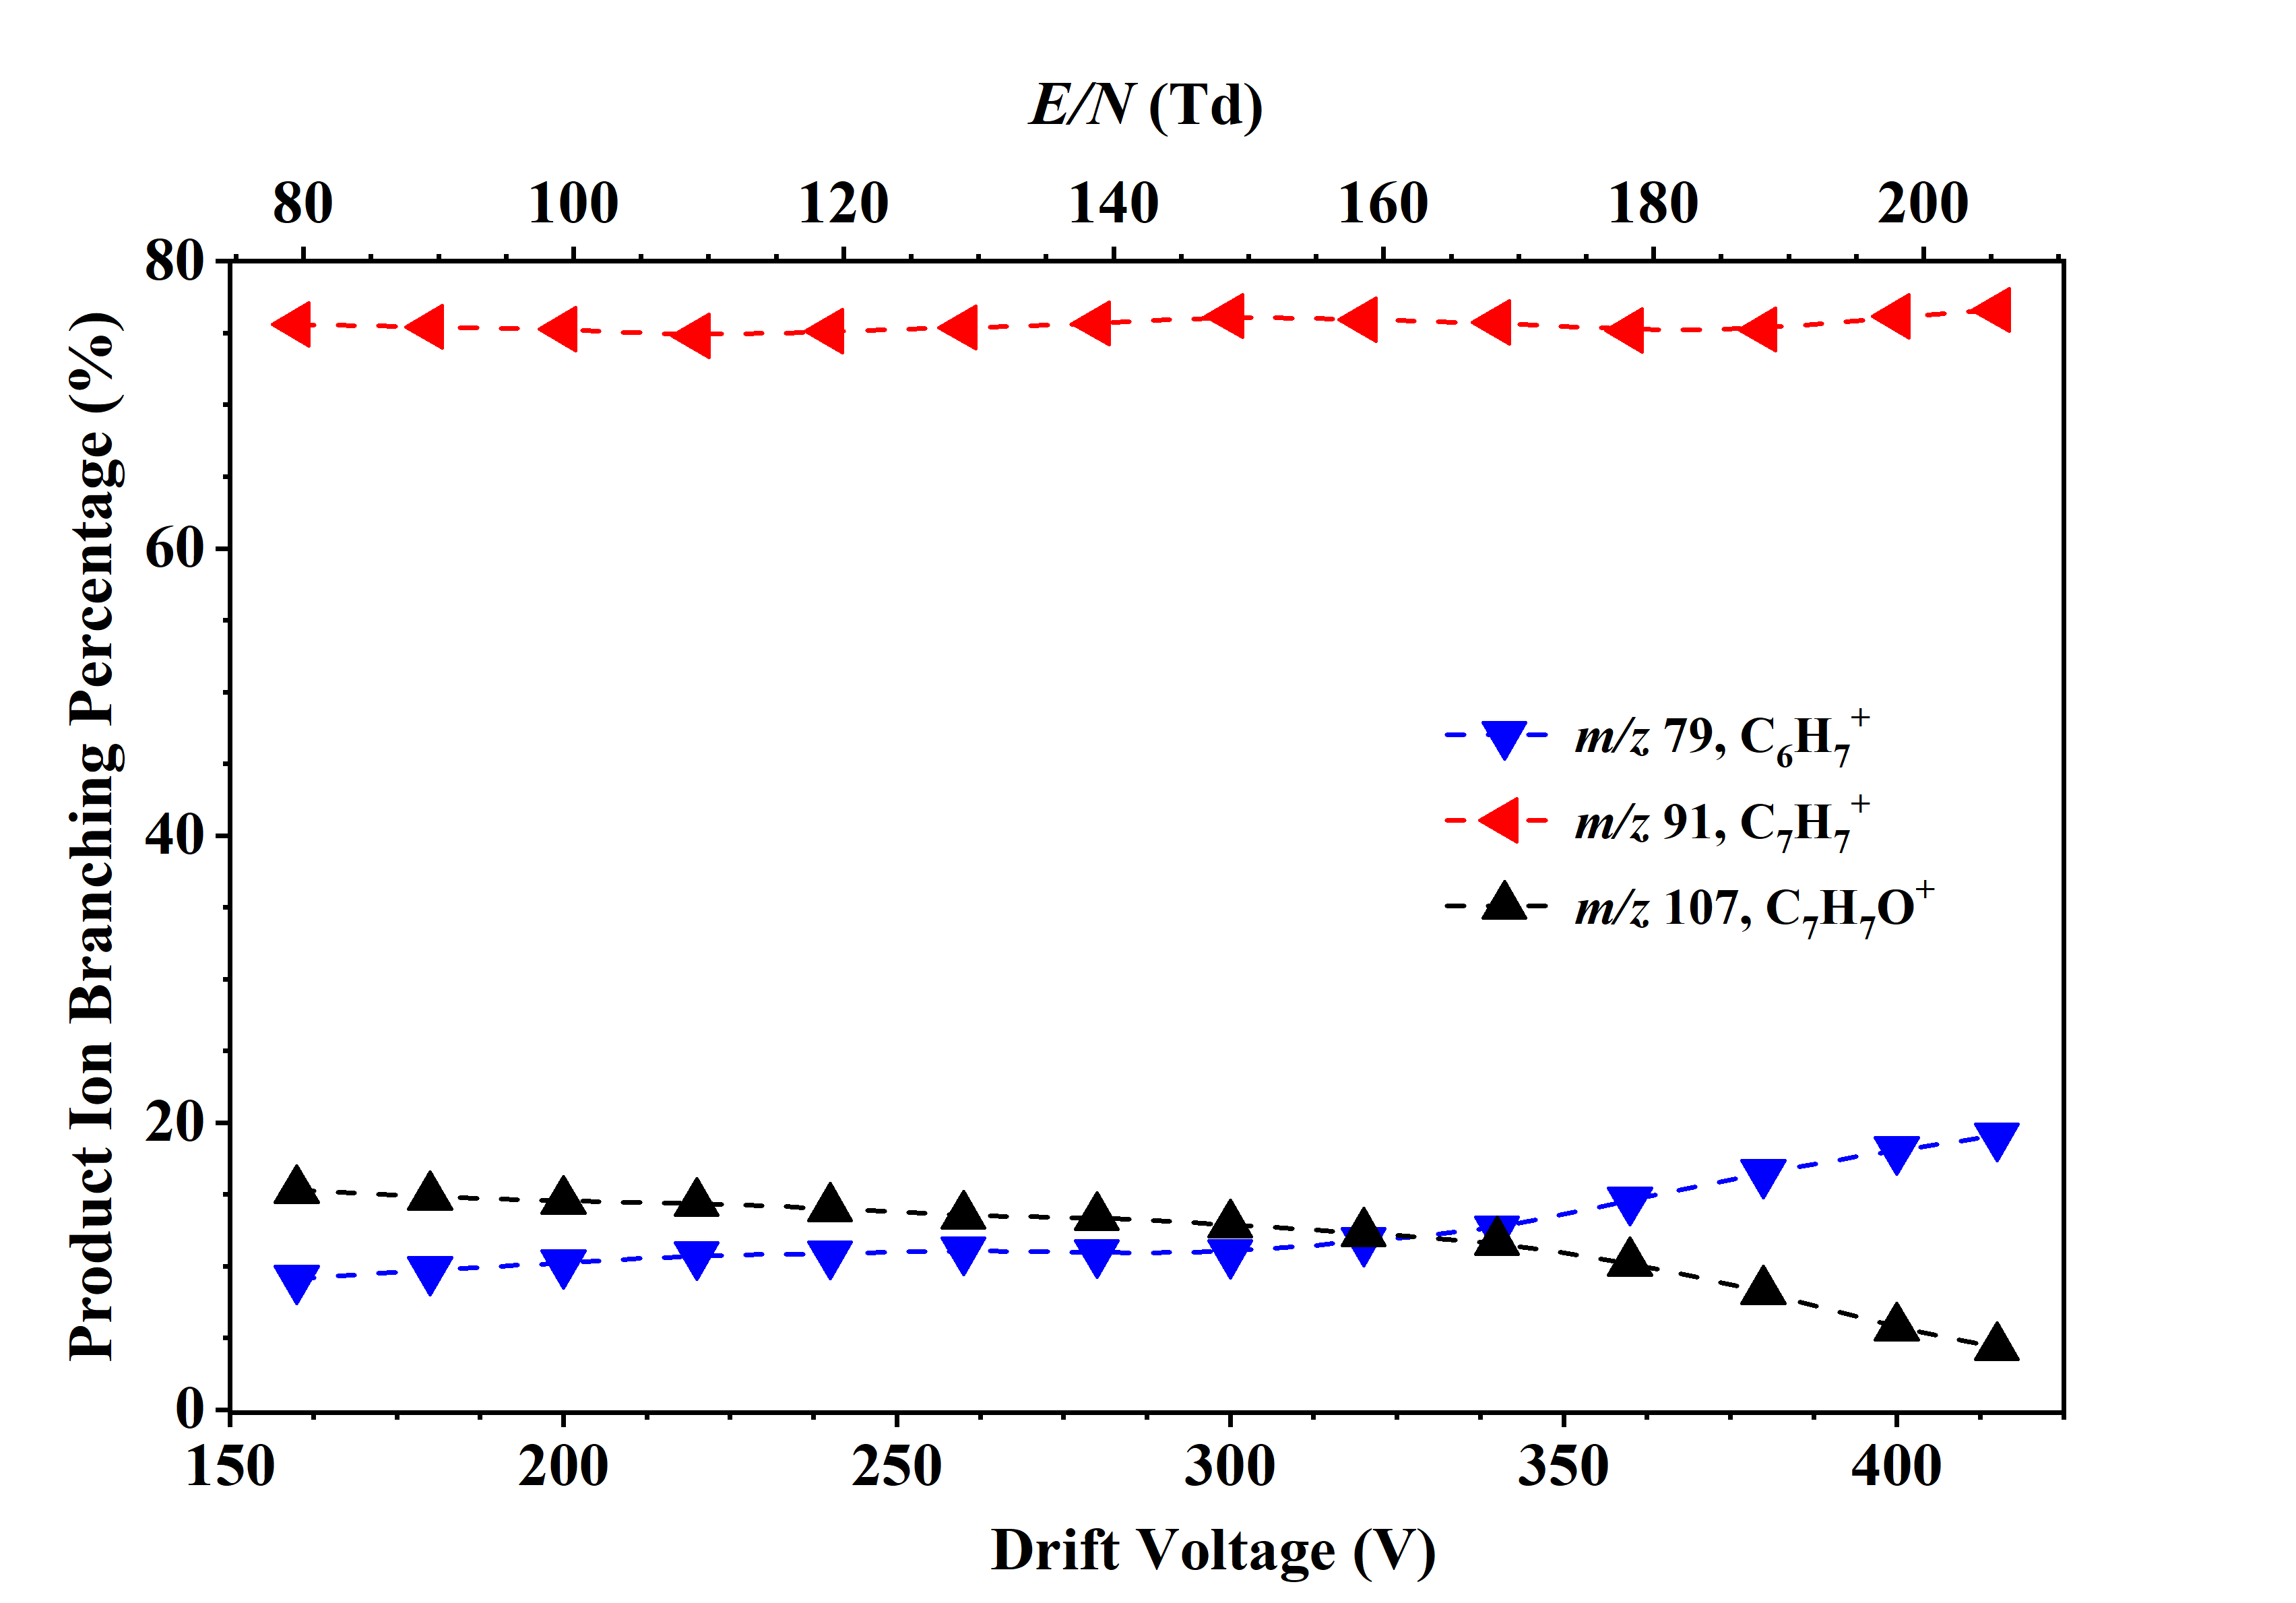
\includegraphics[height=0.4\textheight]{pics/DBeP-BR.png}
\caption{Percentage product ion distribution resulting from the reaction of DBeP with H\textsubscript{3}O\textsuperscript{+} as a function of the drift voltage and the reduced electric field in the range from 80 to 205 Td.}
\label{fig:DBeP_fs}
\end{figure}




\begin{figure}
\centering
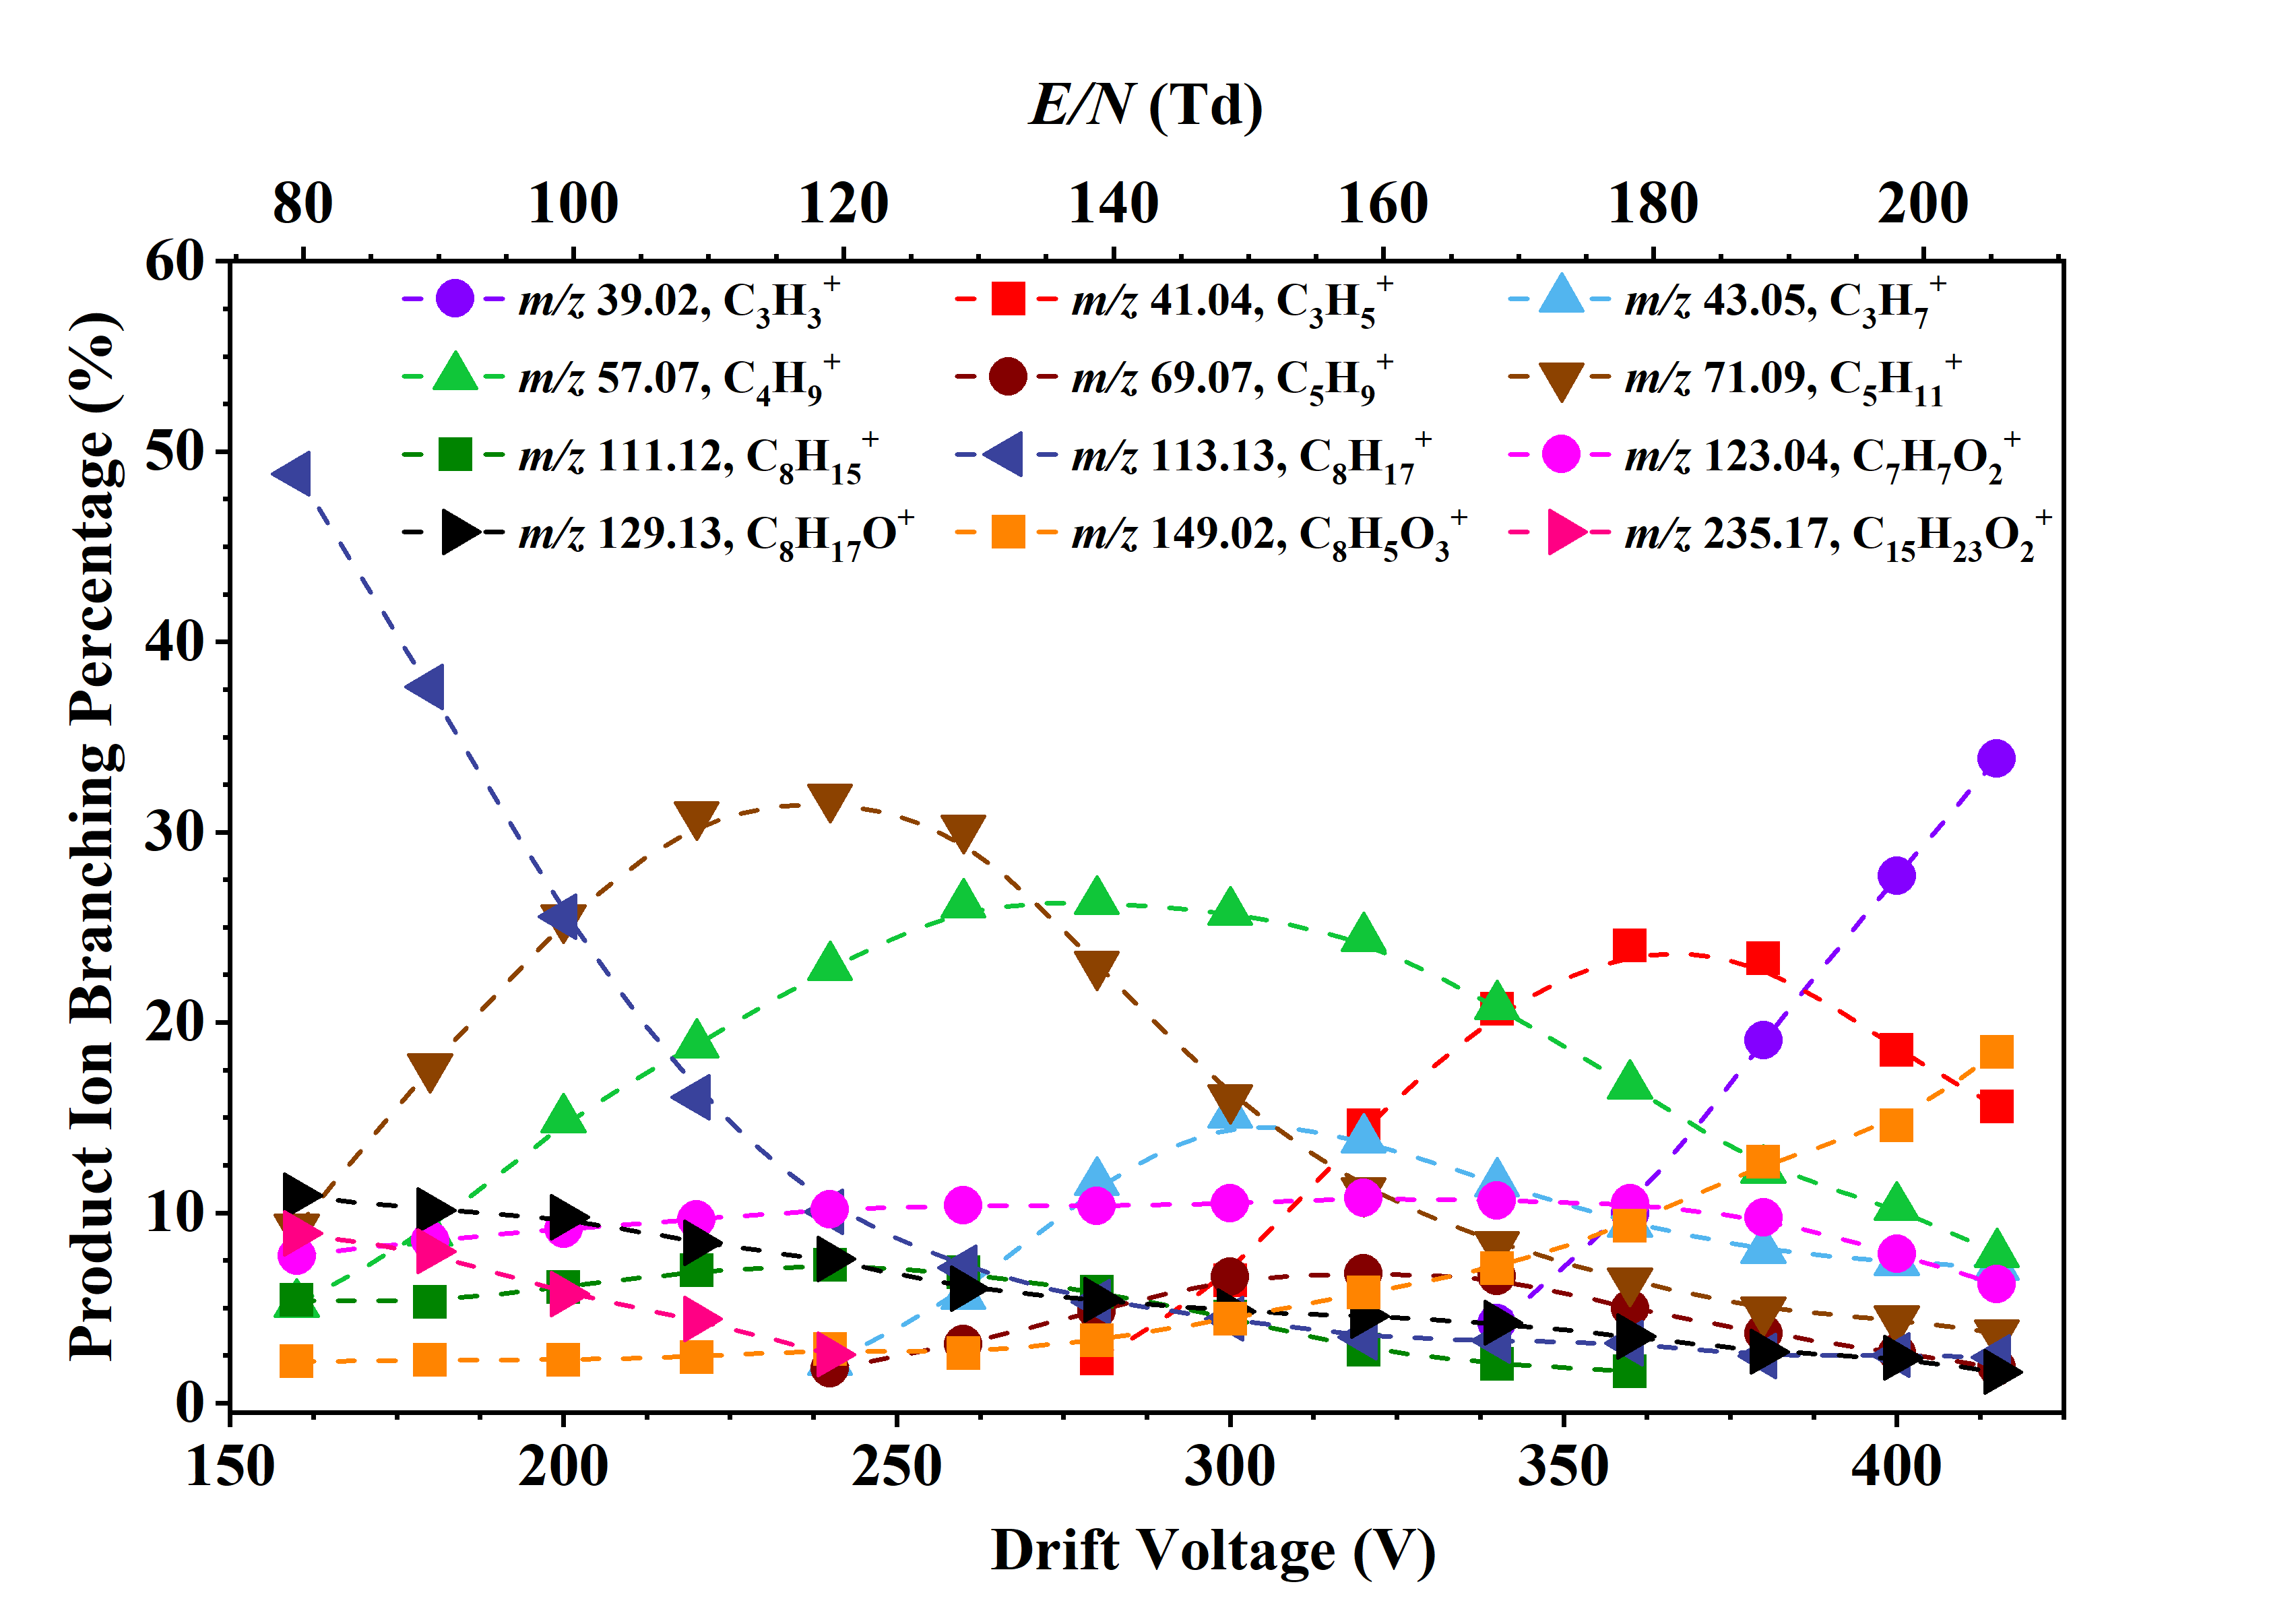
\includegraphics[height=0.4\textheight]{pics/DEHP-BR.png}
\caption{Percentage product ion distribution  resulting from the reaction of DEHP with H\textsubscript{3}O\textsuperscript{+} as a function of the drift voltage and the reduced electric field in the range from 80 to 205 Td.}
\label{fig:DEHP_fs}
\end{figure}






\section{Conclusions}



